         \chapter{Review of Past Work}
    \setcounter{figure}{1}\setcounter{subfigure}{1}\label{m38346}
    \section{Introduction}
            \nopagebreak
%%            \label{m38346*cid2} $ \hspace{-5pt}\begin{array}{cccccccccccc}   \end{array} $ \hspace{2 pt}\raisebox{-5 pt}{
\includegraphics[width=0.5cm]{col11306.imgs/summary_www.png}} {(section shortcode: MG10000 )} \par 
      \label{m38346*id171138}This chapter describes some basic concepts which you have seen in earlier grades and lays the foundation for the remainder of this book. You should feel confident with the content in this chapter, before moving on with the rest of the book.\par 
      \label{m38346*id171143}You can try out your skills on exercises in this chapter and ask your teacher for more questions just like them. You can also try to make up your own questions, solve them and try them out on your classmates to see if you get the same answers.\par 
      \label{m38346*id171149}Practice is the only way to get good at maths!\par 
    \section{What is a number?}
            \nopagebreak
%%            \label{m38346*cid3} $ \hspace{-5pt}\begin{array}{cccccccccccc}   \end{array} $ \hspace{2 pt}\raisebox{-5 pt}{
\includegraphics[width=0.5cm]{col11306.imgs/summary_www.png}} {(section shortcode: MG10001 )} \par 
      \label{m38346*id171500}A number is a way to represent quantity. Numbers are not something that you can touch or hold, because they are not physical. But you can touch three apples, three pencils, three books. You can never just touch three, you can only touch three of something. However, you do not need to see three apples in front of you to know that if you take one apple away, there will be two apples left. You can just think about it. That is your brain representing the apples in numbers and then performing arithmetic on them.\par 
      \label{m38346*id171507}A number represents quantity because we can look at the world around us and
quantify it using numbers. How many minutes? How many kilometers? How
many apples? How much money? How much medicine? These are all questions which can only be answered using numbers to tell us ``how much'' of something we want to measure.\par 
      \label{m38346*id171516}A number can be written in many different ways and it is always best to choose the most appropriate way of writing the number. For example, ``a half'' may be spoken aloud or written in words, but that makes mathematics very difficult and also means that only people who speak the same language as you can understand what you mean. A better way of writing ``a half'' is as a fraction $\frac{1}{2}$ or as a decimal number $0,5$. It is still the same number, no matter which way you write it.\par 
      \label{m38346*id171551}In high school, all the numbers which you will see are called \textsl{real
numbers} and mathematicians use the symbol $\mathbb{R}$ to represent the \textsl{set of all real numbers}, which simply means all of the real numbers. Some of these real numbers can be written in ways that others cannot. Different types of numbers are described in detail in Section 1.12.\par 
    \section{Sets}
            \nopagebreak
%%            \label{m38346*cid4} $ \hspace{-5pt}\begin{array}{cccccccccccc}   \end{array} $ \hspace{2 pt}\raisebox{-5 pt}{
\includegraphics[width=0.5cm]{col11306.imgs/summary_www.png}} {(section shortcode: MG10002 )} \par 
      \label{m38346*id171586}A \textsl{set} is a group of objects with a well-defined criterion for membership. For example, the criterion for belonging to a set of apples, is that the object must be an apple. The set of apples can then be divided into red apples and green apples, but they are all still apples. All the red apples form another set which is a \textsl{sub-set} of the set of apples. A sub-set is part of a set. All the green apples form another sub-set.\par 
      \label{m38346*id171604}Now we come to the idea of a \textbf{union}, which is used to combine things. The symbol for \textbf{union} is $\cup $. Here, we use it to combine two or more intervals. For example, if $x$ is a real number such that $1\lessthan{}x\le 3$ or $6\le x\lessthan{}10$\hspace{1ex}, then the set of all the possible $x$ values is:\par 
      \label{m38346*uid1}\nopagebreak\noindent{}
        \settowidth{\mymathboxwidth}{\begin{equation}
    \left(1,3\right]\cup \left[6,10\right)\tag{1}
      \end{equation}
    }
    \typeout{Columnwidth = \the\columnwidth}\typeout{math as usual width = \the\mymathboxwidth}
    \ifthenelse{\lengthtest{\mymathboxwidth < \columnwidth}}{% if the math fits, do it again, for real
    \begin{equation}
    \left(1,3\right]\cup \left[6,10\right)\tag{1}
      \end{equation}
    }{% else, if it doesn't fit
    \setlength{\mymathboxwidth}{\columnwidth}
      \addtolength{\mymathboxwidth}{-48pt}
    \par\vspace{12pt}\noindent\begin{minipage}{\columnwidth}
    \parbox[t]{\mymathboxwidth}{\large$
    \left(1,3\right]\cup \left[6,10\right)$}\hfill
    \parbox[t]{48pt}{\raggedleft 
    (1)}
    \end{minipage}\vspace{12pt}\par
    }% end of conditional for this bit of math
    \typeout{math as usual width = \the\mymathboxwidth}
      \label{m38346*id171079}where the $\cup $ sign means the union (or combination) of the two intervals. We use the set and interval notation and the symbols described because it is easier than having to write everything out in words.\par 
    \section{Letters and Arithmetic}
            \nopagebreak
%%            \label{m38346*cid5} $ \hspace{-5pt}\begin{array}{cccccccccccc}   \end{array} $ \hspace{2 pt}\raisebox{-5 pt}{
\includegraphics[width=0.5cm]{col11306.imgs/summary_www.png}} {(section shortcode: MG10003 )} \par 
      \label{m38346*id171917}The simplest thing that can be done with numbers is adding, subtracting, multiplying or dividing them. When two numbers are added, subtracted, multiplied or divided, you are performing \textsl{arithmetic}\label{m38346*uid2}\footnote{Arithmetic is derived from the Greek word \textsl{arithmos} meaning \textsl{number}.}. These four basic operations can be performed on any two real numbers.\par 
      \label{m38346*id171947}Mathematics as a language uses special notation to write things down. So instead of:\par 
      \label{m38346*eip-237}one plus one is equal to two\par \label{m38346*id171974}mathematicians write\par 
      \label{m38346*id171980}\nopagebreak\noindent{}
        \settowidth{\mymathboxwidth}{\begin{equation}
    1+1=2\tag{2}
      \end{equation}
    }
    \typeout{Columnwidth = \the\columnwidth}\typeout{math as usual width = \the\mymathboxwidth}
    \ifthenelse{\lengthtest{\mymathboxwidth < \columnwidth}}{% if the math fits, do it again, for real
    \begin{equation}
    1+1=2\tag{2}
      \end{equation}
    }{% else, if it doesn't fit
    \setlength{\mymathboxwidth}{\columnwidth}
      \addtolength{\mymathboxwidth}{-48pt}
    \par\vspace{12pt}\noindent\begin{minipage}{\columnwidth}
    \parbox[t]{\mymathboxwidth}{\large$
    1+1=2$}\hfill
    \parbox[t]{48pt}{\raggedleft 
    (2)}
    \end{minipage}\vspace{12pt}\par
    }% end of conditional for this bit of math
    \typeout{math as usual width = \the\mymathboxwidth}
      \label{m38346*id171999}In earlier grades, place holders were used to indicate missing numbers in an equation.\par 
      \label{m38346*id172003}\nopagebreak\noindent{}
        \settowidth{\mymathboxwidth}{\begin{equation}
    \begin{array}{cc}\hfill 1+\square =2\\ \hfill 4-\square =2\\ \hfill \square +3-2\square =2\end{array}\tag{3}
      \end{equation}
    }
    \typeout{Columnwidth = \the\columnwidth}\typeout{math as usual width = \the\mymathboxwidth}
    \ifthenelse{\lengthtest{\mymathboxwidth < \columnwidth}}{% if the math fits, do it again, for real
    \begin{equation}
    \begin{array}{cc}\hfill 1+\square =2\\ \hfill 4-\square =2\\ \hfill \square +3-2\square =2\end{array}\tag{3}
      \end{equation}
    }{% else, if it doesn't fit
    \setlength{\mymathboxwidth}{\columnwidth}
      \addtolength{\mymathboxwidth}{-48pt}
    \par\vspace{12pt}\noindent\begin{minipage}{\columnwidth}
    \parbox[t]{\mymathboxwidth}{\large$
    1+\square =24-\square =2\square +3-2\square =2$}\hfill
    \parbox[t]{48pt}{\raggedleft 
    (3)}
    \end{minipage}\vspace{12pt}\par
    }% end of conditional for this bit of math
    \typeout{math as usual width = \the\mymathboxwidth}
      \label{m38346*id172068}However, place holders only work well for simple equations. For more advanced mathematical workings, letters are usually used to represent numbers.\par 
      \label{m38346*uid3}\nopagebreak\noindent{}
        \settowidth{\mymathboxwidth}{\begin{equation}
    \begin{array}{cc}\hfill 1+x=2\\ \hfill 4-y=2\\ \hfill z+3-2z=2\end{array}\tag{4}
      \end{equation}
    }
    \typeout{Columnwidth = \the\columnwidth}\typeout{math as usual width = \the\mymathboxwidth}
    \ifthenelse{\lengthtest{\mymathboxwidth < \columnwidth}}{% if the math fits, do it again, for real
    \begin{equation}
    \begin{array}{cc}\hfill 1+x=2\\ \hfill 4-y=2\\ \hfill z+3-2z=2\end{array}\tag{4}
      \end{equation}
    }{% else, if it doesn't fit
    \setlength{\mymathboxwidth}{\columnwidth}
      \addtolength{\mymathboxwidth}{-48pt}
    \par\vspace{12pt}\noindent\begin{minipage}{\columnwidth}
    \parbox[t]{\mymathboxwidth}{\large$
    1+x=24-y=2z+3-2z=2$}\hfill
    \parbox[t]{48pt}{\raggedleft 
    (4)}
    \end{minipage}\vspace{12pt}\par
    }% end of conditional for this bit of math
    \typeout{math as usual width = \the\mymathboxwidth}
      \label{m38346*id172141}These letters are referred to as \textbf{variables}, since they can take on any value depending on what is required. For example, $x=1$ in (4), but $x=26$\hspace{1ex} in $2+x=28$.\par 
      \label{m38346*id172198}A \textbf{constant} has a fixed value. The number 1 is a constant. The \textsl{speed of light} in a vacuum is also a constant which has been defined to be exactly $299 792 458\phantom{\rule{3pt}{0ex}}m\ensuremath{\cdot}s{}^{-1}$ (read metres per second). The speed of light is a big number and it takes up space to always write down the entire number. Therefore, letters are also used to represent some constants. In the case of the speed of light, it is accepted that the letter $c$ represents the speed of light. Such constants represented by letters occur most often in physics and chemistry.\par 
      \label{m38346*id172250}Additionally, letters can be used to describe a situation mathematically. For example, the following equation\par 
      \label{m38346*uid4}\nopagebreak\noindent{}
        \settowidth{\mymathboxwidth}{\begin{equation}
    x+y=z\tag{5}
      \end{equation}
    }
    \typeout{Columnwidth = \the\columnwidth}\typeout{math as usual width = \the\mymathboxwidth}
    \ifthenelse{\lengthtest{\mymathboxwidth < \columnwidth}}{% if the math fits, do it again, for real
    \begin{equation}
    x+y=z\tag{5}
      \end{equation}
    }{% else, if it doesn't fit
    \setlength{\mymathboxwidth}{\columnwidth}
      \addtolength{\mymathboxwidth}{-48pt}
    \par\vspace{12pt}\noindent\begin{minipage}{\columnwidth}
    \parbox[t]{\mymathboxwidth}{\large$
    x+y=z$}\hfill
    \parbox[t]{48pt}{\raggedleft 
    (5)}
    \end{minipage}\vspace{12pt}\par
    }% end of conditional for this bit of math
    \typeout{math as usual width = \the\mymathboxwidth}
      \label{m38346*id172278}can be used to describe the situation of finding how much change can be expected for buying an item. In this equation, $y$ represents the price of the item you are buying, $x$ represents the amount of change you should get back and $z$ is the amount of money given to the cashier. So, if the price is R10 and you gave the cashier R15, then write R15 instead of $z$ and R10 instead of $y$ and the change is then $x$.\par 
      \label{m38346*uid5}\nopagebreak\noindent{}
        \settowidth{\mymathboxwidth}{\begin{equation}
    x+10=15\tag{6}
      \end{equation}
    }
    \typeout{Columnwidth = \the\columnwidth}\typeout{math as usual width = \the\mymathboxwidth}
    \ifthenelse{\lengthtest{\mymathboxwidth < \columnwidth}}{% if the math fits, do it again, for real
    \begin{equation}
    x+10=15\tag{6}
      \end{equation}
    }{% else, if it doesn't fit
    \setlength{\mymathboxwidth}{\columnwidth}
      \addtolength{\mymathboxwidth}{-48pt}
    \par\vspace{12pt}\noindent\begin{minipage}{\columnwidth}
    \parbox[t]{\mymathboxwidth}{\large$
    x+10=15$}\hfill
    \parbox[t]{48pt}{\raggedleft 
    (6)}
    \end{minipage}\vspace{12pt}\par
    }% end of conditional for this bit of math
    \typeout{math as usual width = \the\mymathboxwidth}
      \label{m38346*id172357}We will learn how to ``solve'' this equation towards the end of this chapter.\par 
    \section{Addition and Subtraction}
            \nopagebreak
%%            \label{m38346*cid6} $ \hspace{-5pt}\begin{array}{cccccccccccc}   \end{array} $ \hspace{2 pt}\raisebox{-5 pt}{
\includegraphics[width=0.5cm]{col11306.imgs/summary_www.png}} {(section shortcode: MG10004 )} \par 
      \label{m38346*id172371}Addition ($+$) and subtraction ($-$) are the most basic operations between numbers but they are very closely related to each other. You can think of subtracting as being the opposite of adding since adding a number and then subtracting the same number will not change what you started with. For example, if we start with $a$ and add $b$, then subtract $b$, we will just get back to
$a$ again:\par 
      \label{m38346*uid6}\nopagebreak\noindent{}
        \settowidth{\mymathboxwidth}{\begin{equation}
    \begin{array}{cc}\hfill a+b-b=a\\ \hfill 5+2-2=5\end{array}\tag{7}
      \end{equation}
    }
    \typeout{Columnwidth = \the\columnwidth}\typeout{math as usual width = \the\mymathboxwidth}
    \ifthenelse{\lengthtest{\mymathboxwidth < \columnwidth}}{% if the math fits, do it again, for real
    \begin{equation}
    \begin{array}{cc}\hfill a+b-b=a\\ \hfill 5+2-2=5\end{array}\tag{7}
      \end{equation}
    }{% else, if it doesn't fit
    \setlength{\mymathboxwidth}{\columnwidth}
      \addtolength{\mymathboxwidth}{-48pt}
    \par\vspace{12pt}\noindent\begin{minipage}{\columnwidth}
    \parbox[t]{\mymathboxwidth}{\large$
    a+b-b=a5+2-2=5$}\hfill
    \parbox[t]{48pt}{\raggedleft 
    (7)}
    \end{minipage}\vspace{12pt}\par
    }% end of conditional for this bit of math
    \typeout{math as usual width = \the\mymathboxwidth}
      \label{m38346*id172463}If we look at a number line, then addition means that we move to the right and subtraction means that we move to the left.\par 
      \label{m38346*id172468}The order in which numbers are added does not matter, but the order in which numbers are subtracted does matter. This means that:\par 
      \label{m38346*uid7}\nopagebreak\noindent{}\settowidth{\mymathboxwidth}{\begin{equation}
    \begin{array}{ccc}\hfill a+b& =& b+a\hfill \\ \hfill a-b& \ne & b-a\mathrm{if}\phantom{\rule{3pt}{0ex}}\mathrm{a}\ne \mathrm{b}\hfill \end{array}\tag{8}
      \end{equation}
    }
    \typeout{Columnwidth = \the\columnwidth}\typeout{math as usual width = \the\mymathboxwidth}
    \ifthenelse{\lengthtest{\mymathboxwidth < \columnwidth}}{% if the math fits, do it again, for real
    \begin{equation}
    \begin{array}{ccc}\hfill a+b& =& b+a\hfill \\ \hfill a-b& \ne & b-a\mathrm{if}\phantom{\rule{3pt}{0ex}}\mathrm{a}\ne \mathrm{b}\hfill \end{array}\tag{8}
      \end{equation}
    }{% else, if it doesn't fit
    \setlength{\mymathboxwidth}{\columnwidth}
      \addtolength{\mymathboxwidth}{-48pt}
    \par\vspace{12pt}\noindent\begin{minipage}{\columnwidth}
    \parbox[t]{\mymathboxwidth}{\large$
    a+b=b+aa-b\ne b-a\mathrm{if}\phantom{\rule{3pt}{0ex}}\mathrm{a}\ne \mathrm{b}$}\hfill
    \parbox[t]{48pt}{\raggedleft 
    (8)}
    \end{minipage}\vspace{12pt}\par
    }% end of conditional for this bit of math
    \typeout{math as usual width = \the\mymathboxwidth}
      \label{m38346*id172553}The sign $\ne $ means ``is not equal to''. For example, $2+3=5$ and $3+2=5$, but $5-3=2$ and $3-5=-2$. $-2$ is a negative number, which is explained in detail in "Negative Numbers" (Section~: Negative Numbers).\par 
\label{m38346*secfhsst!!!underscore!!!id341}
            \subsection{  Commutativity for Addition }
            \nopagebreak
      \label{m38346*id172661}The fact that $a+b=b+a$, is known as the
\textsl{commutative} property for addition. \par 
    \section{Multiplication and Division}
            \nopagebreak
%%            \label{m38346*cid7} $ \hspace{-5pt}\begin{array}{cccccccccccc}   \end{array} $ \hspace{2 pt}\raisebox{-5 pt}{
\includegraphics[width=0.5cm]{col11306.imgs/summary_www.png}} {(section shortcode: MG10005 )} \par 
      \label{m38346*id172708}Just like addition and subtraction, multiplication ($\ensuremath{\times}$, $\ensuremath{\cdot}$) and
division ($÷$, /) are opposites of each other. Multiplying by a number and
then dividing by the same number gets us back to the start again:\par 
      \label{m38346*uid8}\nopagebreak\noindent{}
        \settowidth{\mymathboxwidth}{\begin{equation}
    \begin{array}{cc}\hfill a\ensuremath{\times}b÷b=a\\ \hfill 5\ensuremath{\times}4÷4=5\end{array}\tag{9}
      \end{equation}
    }
    \typeout{Columnwidth = \the\columnwidth}\typeout{math as usual width = \the\mymathboxwidth}
    \ifthenelse{\lengthtest{\mymathboxwidth < \columnwidth}}{% if the math fits, do it again, for real
    \begin{equation}
    \begin{array}{cc}\hfill a\ensuremath{\times}b÷b=a\\ \hfill 5\ensuremath{\times}4÷4=5\end{array}\tag{9}
      \end{equation}
    }{% else, if it doesn't fit
    \setlength{\mymathboxwidth}{\columnwidth}
      \addtolength{\mymathboxwidth}{-48pt}
    \par\vspace{12pt}\noindent\begin{minipage}{\columnwidth}
    \parbox[t]{\mymathboxwidth}{\large$
    a\ensuremath{\times}b÷b=a5\ensuremath{\times}4÷4=5$}\hfill
    \parbox[t]{48pt}{\raggedleft 
    (9)}
    \end{minipage}\vspace{12pt}\par
    }% end of conditional for this bit of math
    \typeout{math as usual width = \the\mymathboxwidth}
      \label{m38346*id172791}Sometimes you will see a multiplication of letters as a dot or
without any symbol. Don't worry, its exactly the same thing. Mathematicians are
efficient and like to write things in the shortest, neatest way possible.\par 
      \label{m38346*uid9}\nopagebreak\noindent{}
        \settowidth{\mymathboxwidth}{\begin{equation}
    \begin{array}{ccc}\hfill abc& =& a\ensuremath{\times}b\ensuremath{\times}c\hfill \\ \hfill a\ensuremath{\cdot}b\ensuremath{\cdot}c& =& a\ensuremath{\times}b\ensuremath{\times}c\hfill \end{array}\tag{10}
      \end{equation}
    }
    \typeout{Columnwidth = \the\columnwidth}\typeout{math as usual width = \the\mymathboxwidth}
    \ifthenelse{\lengthtest{\mymathboxwidth < \columnwidth}}{% if the math fits, do it again, for real
    \begin{equation}
    \begin{array}{ccc}\hfill abc& =& a\ensuremath{\times}b\ensuremath{\times}c\hfill \\ \hfill a\ensuremath{\cdot}b\ensuremath{\cdot}c& =& a\ensuremath{\times}b\ensuremath{\times}c\hfill \end{array}\tag{10}
      \end{equation}
    }{% else, if it doesn't fit
    \setlength{\mymathboxwidth}{\columnwidth}
      \addtolength{\mymathboxwidth}{-48pt}
    \par\vspace{12pt}\noindent\begin{minipage}{\columnwidth}
    \parbox[t]{\mymathboxwidth}{\large$
    abc=a\ensuremath{\times}b\ensuremath{\times}ca\ensuremath{\cdot}b\ensuremath{\cdot}c=a\ensuremath{\times}b\ensuremath{\times}c$}\hfill
    \parbox[t]{48pt}{\raggedleft 
    (10)}
    \end{minipage}\vspace{12pt}\par
    }% end of conditional for this bit of math
    \typeout{math as usual width = \the\mymathboxwidth}
      \label{m38346*id172875}It is usually neater to write known numbers to the left, and letters to the
right. So although $4x$ and $x4$ are the same thing, it looks better to
write $4x$. In this case, the ``4'' is a constant that is referred to as the
\textsl{coefficient} of $x$.\par 
\label{m38346*secfhsst!!!underscore!!!id440}
            \subsection{  Commutativity for Multiplication }
            \nopagebreak
      \label{m38346*id172933}The fact that $ab=ba$ is known as
the \textsl{commutative} property of multiplication. Therefore, both addition
and multiplication are described as commutative operations. \par 
    \section{Brackets}
            \nopagebreak
%%            \label{m38346*cid8} $ \hspace{-5pt}\begin{array}{cccccccccccc}   \end{array} $ \hspace{2 pt}\raisebox{-5 pt}{
\includegraphics[width=0.5cm]{col11306.imgs/summary_www.png}} {(section shortcode: MG10006 )} \par 
      \label{m38346*id172976}Brackets\label{m38346*uid10}\footnote{Sometimes people say ``parentheses'' instead of ``brackets''.}
in mathematics are used to show the order in which you must do things. This is
important as you can get different answers depending on the order in which you
do things. For example:\par 
      \label{m38346*uid11}\nopagebreak\noindent{}
        \settowidth{\mymathboxwidth}{\begin{equation}
    \left(5\ensuremath{\times}5\right)+20=45\tag{11}
      \end{equation}
    }
    \typeout{Columnwidth = \the\columnwidth}\typeout{math as usual width = \the\mymathboxwidth}
    \ifthenelse{\lengthtest{\mymathboxwidth < \columnwidth}}{% if the math fits, do it again, for real
    \begin{equation}
    \left(5\ensuremath{\times}5\right)+20=45\tag{11}
      \end{equation}
    }{% else, if it doesn't fit
    \setlength{\mymathboxwidth}{\columnwidth}
      \addtolength{\mymathboxwidth}{-48pt}
    \par\vspace{12pt}\noindent\begin{minipage}{\columnwidth}
    \parbox[t]{\mymathboxwidth}{\large$
    \left(5\ensuremath{\times}5\right)+20=45$}\hfill
    \parbox[t]{48pt}{\raggedleft 
    (11)}
    \end{minipage}\vspace{12pt}\par
    }% end of conditional for this bit of math
    \typeout{math as usual width = \the\mymathboxwidth}
      \label{m38346*id173024}whereas\par 
      \label{m38346*uid12}\nopagebreak\noindent{}
        \settowidth{\mymathboxwidth}{\begin{equation}
    5\ensuremath{\times}\left(5+20\right)=125\tag{12}
      \end{equation}
    }
    \typeout{Columnwidth = \the\columnwidth}\typeout{math as usual width = \the\mymathboxwidth}
    \ifthenelse{\lengthtest{\mymathboxwidth < \columnwidth}}{% if the math fits, do it again, for real
    \begin{equation}
    5\ensuremath{\times}\left(5+20\right)=125\tag{12}
      \end{equation}
    }{% else, if it doesn't fit
    \setlength{\mymathboxwidth}{\columnwidth}
      \addtolength{\mymathboxwidth}{-48pt}
    \par\vspace{12pt}\noindent\begin{minipage}{\columnwidth}
    \parbox[t]{\mymathboxwidth}{\large$
    5\ensuremath{\times}\left(5+20\right)=125$}\hfill
    \parbox[t]{48pt}{\raggedleft 
    (12)}
    \end{minipage}\vspace{12pt}\par
    }% end of conditional for this bit of math
    \typeout{math as usual width = \the\mymathboxwidth}
      \label{m38346*id173063}If there are no brackets, you should always do multiplications and
divisions first and then additions and subtractions\label{m38346*uid13}\footnote{Multiplying and
dividing can be performed in any order as it doesn't matter. Likewise it
doesn't matter which order you do addition and subtraction. Just as long as
you do any $\ensuremath{\times}÷$ before any $+-$.}. You can always put your own brackets
into equations using this rule to make things easier for yourself, for example:\par 
      \label{m38346*uid14}\nopagebreak\noindent{}
        \settowidth{\mymathboxwidth}{\begin{equation}
    \begin{array}{ccc}\hfill a\ensuremath{\times}b+c÷d& =& \left(a\ensuremath{\times}b\right)+\left(c÷d\right)\hfill \\ \hfill 5\ensuremath{\times}5+20÷4& =& \left(5\ensuremath{\times}5\right)+\left(20÷4\right)\hfill \end{array}\tag{13}
      \end{equation}
    }
    \typeout{Columnwidth = \the\columnwidth}\typeout{math as usual width = \the\mymathboxwidth}
    \ifthenelse{\lengthtest{\mymathboxwidth < \columnwidth}}{% if the math fits, do it again, for real
    \begin{equation}
    \begin{array}{ccc}\hfill a\ensuremath{\times}b+c÷d& =& \left(a\ensuremath{\times}b\right)+\left(c÷d\right)\hfill \\ \hfill 5\ensuremath{\times}5+20÷4& =& \left(5\ensuremath{\times}5\right)+\left(20÷4\right)\hfill \end{array}\tag{13}
      \end{equation}
    }{% else, if it doesn't fit
    \setlength{\mymathboxwidth}{\columnwidth}
      \addtolength{\mymathboxwidth}{-48pt}
    \par\vspace{12pt}\noindent\begin{minipage}{\columnwidth}
    \parbox[t]{\mymathboxwidth}{\large$
    a\ensuremath{\times}b+c÷d=\left(a\ensuremath{\times}b\right)+\left(c÷d\right)5\ensuremath{\times}5+20÷4=\left(5\ensuremath{\times}5\right)+\left(20÷4\right)$}\hfill
    \parbox[t]{48pt}{\raggedleft 
    (13)}
    \end{minipage}\vspace{12pt}\par
    }% end of conditional for this bit of math
    \typeout{math as usual width = \the\mymathboxwidth}
      \label{m38346*id173227}If you see a multiplication outside a bracket like this\par 
      \label{m38346*uid15}\nopagebreak\noindent{}
        \settowidth{\mymathboxwidth}{\begin{equation}
    \begin{array}{cc}\hfill a\left(b+c\right)\\ \hfill 3\left(4-3\right)\end{array}\tag{14}
      \end{equation}
    }
    \typeout{Columnwidth = \the\columnwidth}\typeout{math as usual width = \the\mymathboxwidth}
    \ifthenelse{\lengthtest{\mymathboxwidth < \columnwidth}}{% if the math fits, do it again, for real
    \begin{equation}
    \begin{array}{cc}\hfill a\left(b+c\right)\\ \hfill 3\left(4-3\right)\end{array}\tag{14}
      \end{equation}
    }{% else, if it doesn't fit
    \setlength{\mymathboxwidth}{\columnwidth}
      \addtolength{\mymathboxwidth}{-48pt}
    \par\vspace{12pt}\noindent\begin{minipage}{\columnwidth}
    \parbox[t]{\mymathboxwidth}{\large$
    a\left(b+c\right)3\left(4-3\right)$}\hfill
    \parbox[t]{48pt}{\raggedleft 
    (14)}
    \end{minipage}\vspace{12pt}\par
    }% end of conditional for this bit of math
    \typeout{math as usual width = \the\mymathboxwidth}
      \label{m38346*id173283}then it means you have to multiply each part inside the bracket by the number
outside\par 
      \label{m38346*uid16}\nopagebreak\noindent{}
        \settowidth{\mymathboxwidth}{\begin{equation}
    \begin{array}{ccc}\hfill a\left(b+c\right)& =& ab+ac\hfill \\ \hfill 3\left(4-3\right)& =& 3\ensuremath{\times}4-3\ensuremath{\times}3=12-9=3\hfill \end{array}\tag{15}
      \end{equation}
    }
    \typeout{Columnwidth = \the\columnwidth}\typeout{math as usual width = \the\mymathboxwidth}
    \ifthenelse{\lengthtest{\mymathboxwidth < \columnwidth}}{% if the math fits, do it again, for real
    \begin{equation}
    \begin{array}{ccc}\hfill a\left(b+c\right)& =& ab+ac\hfill \\ \hfill 3\left(4-3\right)& =& 3\ensuremath{\times}4-3\ensuremath{\times}3=12-9=3\hfill \end{array}\tag{15}
      \end{equation}
    }{% else, if it doesn't fit
    \setlength{\mymathboxwidth}{\columnwidth}
      \addtolength{\mymathboxwidth}{-48pt}
    \par\vspace{12pt}\noindent\begin{minipage}{\columnwidth}
    \parbox[t]{\mymathboxwidth}{\large$
    a\left(b+c\right)=ab+ac3\left(4-3\right)=3\ensuremath{\times}4-3\ensuremath{\times}3=12-9=3$}\hfill
    \parbox[t]{48pt}{\raggedleft 
    (15)}
    \end{minipage}\vspace{12pt}\par
    }% end of conditional for this bit of math
    \typeout{math as usual width = \the\mymathboxwidth}
      \label{m38346*id173397}unless you can simplify everything inside the bracket into a single term. In
fact, in the above example, it would have been smarter to have done this\par 
      \label{m38346*uid17}\nopagebreak\noindent{}
        \settowidth{\mymathboxwidth}{\begin{equation}
    3\left(4-3\right)=3\ensuremath{\times}\left(1\right)=3\tag{16}
      \end{equation}
    }
    \typeout{Columnwidth = \the\columnwidth}\typeout{math as usual width = \the\mymathboxwidth}
    \ifthenelse{\lengthtest{\mymathboxwidth < \columnwidth}}{% if the math fits, do it again, for real
    \begin{equation}
    3\left(4-3\right)=3\ensuremath{\times}\left(1\right)=3\tag{16}
      \end{equation}
    }{% else, if it doesn't fit
    \setlength{\mymathboxwidth}{\columnwidth}
      \addtolength{\mymathboxwidth}{-48pt}
    \par\vspace{12pt}\noindent\begin{minipage}{\columnwidth}
    \parbox[t]{\mymathboxwidth}{\large$
    3\left(4-3\right)=3\ensuremath{\times}\left(1\right)=3$}\hfill
    \parbox[t]{48pt}{\raggedleft 
    (16)}
    \end{minipage}\vspace{12pt}\par
    }% end of conditional for this bit of math
    \typeout{math as usual width = \the\mymathboxwidth}
      \label{m38346*id173448}It can happen with letters too\par 
      \label{m38346*uid18}\nopagebreak\noindent{}
        \settowidth{\mymathboxwidth}{\begin{equation}
    3\left(4a-3a\right)=3\ensuremath{\times}\left(a\right)=3a\tag{17}
      \end{equation}
    }
    \typeout{Columnwidth = \the\columnwidth}\typeout{math as usual width = \the\mymathboxwidth}
    \ifthenelse{\lengthtest{\mymathboxwidth < \columnwidth}}{% if the math fits, do it again, for real
    \begin{equation}
    3\left(4a-3a\right)=3\ensuremath{\times}\left(a\right)=3a\tag{17}
      \end{equation}
    }{% else, if it doesn't fit
    \setlength{\mymathboxwidth}{\columnwidth}
      \addtolength{\mymathboxwidth}{-48pt}
    \par\vspace{12pt}\noindent\begin{minipage}{\columnwidth}
    \parbox[t]{\mymathboxwidth}{\large$
    3\left(4a-3a\right)=3\ensuremath{\times}\left(a\right)=3a$}\hfill
    \parbox[t]{48pt}{\raggedleft 
    (17)}
    \end{minipage}\vspace{12pt}\par
    }% end of conditional for this bit of math
    \typeout{math as usual width = \the\mymathboxwidth}
\label{m38346*secfhsst!!!underscore!!!id698}
            \subsection{  Distributivity }
            \nopagebreak
      \label{m38346*id173510}The fact that $a\left(b+c\right)=ab+ac$ is known as the
\textsl{distributive} property. \par 
      \label{m38346*id173561}If there are two brackets multiplied by each other, then you can do it one step
at a time:\par 
      \label{m38346*uid19}\nopagebreak\noindent{}
        \settowidth{\mymathboxwidth}{\begin{equation}
    \begin{array}{ccc}\hfill \left(a+b\right)\left(c+d\right)& =& a\left(c+d\right)+b\left(c+d\right)\hfill \\ \hfill & =& ac+ad+bc+bd\hfill \\ \hfill \left(a+3\right)\left(4+d\right)& =& a\left(4+d\right)+3\left(4+d\right)\hfill \\ \hfill & =& 4a+ad+12+3d\hfill \end{array}\tag{18}
      \end{equation}
    }
    \typeout{Columnwidth = \the\columnwidth}\typeout{math as usual width = \the\mymathboxwidth}
    \ifthenelse{\lengthtest{\mymathboxwidth < \columnwidth}}{% if the math fits, do it again, for real
    \begin{equation}
    \begin{array}{ccc}\hfill \left(a+b\right)\left(c+d\right)& =& a\left(c+d\right)+b\left(c+d\right)\hfill \\ \hfill & =& ac+ad+bc+bd\hfill \\ \hfill \left(a+3\right)\left(4+d\right)& =& a\left(4+d\right)+3\left(4+d\right)\hfill \\ \hfill & =& 4a+ad+12+3d\hfill \end{array}\tag{18}
      \end{equation}
    }{% else, if it doesn't fit
    \setlength{\mymathboxwidth}{\columnwidth}
      \addtolength{\mymathboxwidth}{-48pt}
    \par\vspace{12pt}\noindent\begin{minipage}{\columnwidth}
    \parbox[t]{\mymathboxwidth}{\large$
    \left(a+b\right)\left(c+d\right)=a\left(c+d\right)+b\left(c+d\right)=ac+ad+bc+bd\left(a+3\right)\left(4+d\right)=a\left(4+d\right)+3\left(4+d\right)=4a+ad+12+3d$}\hfill
    \parbox[t]{48pt}{\raggedleft 
    (18)}
    \end{minipage}\vspace{12pt}\par
    }% end of conditional for this bit of math
    \typeout{math as usual width = \the\mymathboxwidth}
    \section{Negative Numbers}
            \nopagebreak
%%            \label{m38346*cid9} $ \hspace{-5pt}\begin{array}{cccccccccccc}   \end{array} $ \hspace{2 pt}\raisebox{-5 pt}{
\includegraphics[width=0.5cm]{col11306.imgs/summary_www.png}} {(section shortcode: MG10007 )} \par 
      \label{m38346*uid20}
            \subsection{ What is a negative number?}
            \nopagebreak
        \label{m38346*id173795}Negative numbers can be very confusing to begin with, but there is nothing to be
afraid of. The numbers that are used most often are greater than zero. These
numbers are known as \textsl{positive numbers}.\par 
        \label{m38346*id173805}A negative number is a number that is less than zero. So, if we were to
take a positive number $a$ and subtract it from zero, the answer would be the
negative of $a$.\par 
        \label{m38346*id173828}\nopagebreak\noindent{}
          \settowidth{\mymathboxwidth}{\begin{equation}
    0-a=-a\tag{19}
      \end{equation}
    }
    \typeout{Columnwidth = \the\columnwidth}\typeout{math as usual width = \the\mymathboxwidth}
    \ifthenelse{\lengthtest{\mymathboxwidth < \columnwidth}}{% if the math fits, do it again, for real
    \begin{equation}
    0-a=-a\tag{19}
      \end{equation}
    }{% else, if it doesn't fit
    \setlength{\mymathboxwidth}{\columnwidth}
      \addtolength{\mymathboxwidth}{-48pt}
    \par\vspace{12pt}\noindent\begin{minipage}{\columnwidth}
    \parbox[t]{\mymathboxwidth}{\large$
    0-a=-a$}\hfill
    \parbox[t]{48pt}{\raggedleft 
    (19)}
    \end{minipage}\vspace{12pt}\par
    }% end of conditional for this bit of math
    \typeout{math as usual width = \the\mymathboxwidth}
        \label{m38346*id173850}On a number line, a negative number appears to the left of zero and a positive
number appears to the right of zero.\par 
    \setcounter{subfigure}{0}
	\begin{figure}[H] % horizontal\label{m38346*uid21}
    \begin{center}
    \rule[.1in]{\figurerulewidth}{.005in} \\
        \label{m38346*uid21!!!underscore!!!media}\label{m38346*uid21!!!underscore!!!printimage}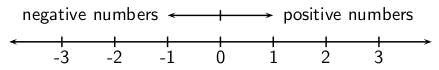
\includegraphics[width=300px]{col11306.imgs/m38346_MG10C2_001.png} % m38346;MG10C2\_001.png;;;6.0;8.5;
      \vspace{2pt}
    \vspace{\rubberspace}\par \begin{cnxcaption}
	  \small \textbf{Figure 1: }On the number line, numbers increase towards the right and decrease
towards the left. Positive numbers appear to the right of zero and negative
numbers appear to the left of zero.
	\end{cnxcaption}
    \vspace{.1in}
    \rule[.1in]{\figurerulewidth}{.005in} \\
    \end{center}
 \end{figure}       
      \label{m38346*uid22}
            \subsection{ Working with Negative Numbers}
            \nopagebreak
        \label{m38346*id173878}When you are adding a negative number, it is the same as subtracting that number
if it were positive. Likewise, if you subtract a negative number, it is the same
as adding the number if it were positive. Numbers are either positive or
negative and we call this their \textsl{s}ign. A positive number has a positive
sign ($+$) and a negative number has a negative sign ($-$).\par 
        \label{m38346*id173907}Subtraction is actually the same as adding a \textsl{negative number}.\par 
        \label{m38346*id173916}In this example, $a$ and $b$ are positive numbers, but $-b$ is a negative number\par 
        \label{m38346*uid23}\nopagebreak\noindent{}
          \settowidth{\mymathboxwidth}{\begin{equation}
    \begin{array}{cc}\hfill a-b=a+\left(-b\right)\\ \hfill 5-3=5+\left(-3\right)\end{array}\tag{20}
      \end{equation}
    }
    \typeout{Columnwidth = \the\columnwidth}\typeout{math as usual width = \the\mymathboxwidth}
    \ifthenelse{\lengthtest{\mymathboxwidth < \columnwidth}}{% if the math fits, do it again, for real
    \begin{equation}
    \begin{array}{cc}\hfill a-b=a+\left(-b\right)\\ \hfill 5-3=5+\left(-3\right)\end{array}\tag{20}
      \end{equation}
    }{% else, if it doesn't fit
    \setlength{\mymathboxwidth}{\columnwidth}
      \addtolength{\mymathboxwidth}{-48pt}
    \par\vspace{12pt}\noindent\begin{minipage}{\columnwidth}
    \parbox[t]{\mymathboxwidth}{\large$
    a-b=a+\left(-b\right)5-3=5+\left(-3\right)$}\hfill
    \parbox[t]{48pt}{\raggedleft 
    (20)}
    \end{minipage}\vspace{12pt}\par
    }% end of conditional for this bit of math
    \typeout{math as usual width = \the\mymathboxwidth}
        \label{m38346*id174020}So, this means that subtraction is simply a short-cut for adding a negative
number and instead of writing $a+\left(-b\right)$, we write $a-b$. This also means that
$-b+a$ is the same as $a-b$. Now, which do you find easier to work out?\par 
        \label{m38346*id174090}Most people find that the first way is a bit more difficult to work out than the
second way. For example, most people find $12-3$ a lot easier to work out than
$-3+12$, even though they are the same thing. So $a-b$, which looks neater and
requires less writing is the accepted way of writing subtractions.\par 
        \label{m38346*id174140}Table 1 shows how to calculate the sign of the answer when
you multiply two numbers together. The first column shows the sign of the first
number, the second column gives the sign of the second number and the third
column shows what sign the answer will be.\par 
    % \textbf{m38346*uid24}\par
          \begin{table}
    % \begin{table}[H]
    % \\ '' '0'
        \begin{center}
      \label{m38346*uid24}
    \noindent
    \tabletail{%
        \hline
        \multicolumn{3}{|p{\mytableboxwidth}|}{\raggedleft \small \sl continued on next page}\\
        \hline
      }
      \tablelasttail{}
      \begin{xtabular}[t]{|l|l|l|}\hline
                  $a$
                 &
                  $b$
                 &
        $a\ensuremath{\times}b$ or $a÷b$% make-rowspan-placeholders
     \tabularnewline\cline{1-1}\cline{2-2}\cline{3-3}
      %--------------------------------------------------------------------
                  $+$
                 &
                  $+$
                 &
                  $+$
                % make-rowspan-placeholders
     \tabularnewline\cline{1-1}\cline{2-2}\cline{3-3}
      %--------------------------------------------------------------------
                  $+$
                 &
                  $-$
                 &
                  $-$
                % make-rowspan-placeholders
     \tabularnewline\cline{1-1}\cline{2-2}\cline{3-3}
      %--------------------------------------------------------------------
                  $-$
                 &
                  $+$
                 &
                  $-$
                % make-rowspan-placeholders
     \tabularnewline\cline{1-1}\cline{2-2}\cline{3-3}
      %--------------------------------------------------------------------
                  $-$
                 &
                  $-$
                 &
                  $+$
                % make-rowspan-placeholders
     \tabularnewline\cline{1-1}\cline{2-2}\cline{3-3}
      %--------------------------------------------------------------------
    \end{xtabular}
      \end{center}
    \begin{center}{\small\bfseries Table 1}: Table of signs for multiplying or dividing two numbers.\end{center}
    \begin{caption}{\small\bfseries Table 1}: Table of signs for multiplying or dividing two numbers.\end{caption}
\end{table}
    \par
        \label{m38346*id174425}So multiplying or dividing a negative number by a positive number always gives
you a negative number, whereas multiplying or dividing numbers which have the
same sign always gives a positive number. For example, $2\ensuremath{\times}3=6$ and
$-2\ensuremath{\times}-3=6$, but $-2\ensuremath{\times}3=-6$ and $2\ensuremath{\times}-3=-6$.\par 
        \label{m38346*id174517}Adding numbers works slightly differently (see Table 2). The first column shows the sign of the first number, the
second column gives the sign of the second number and the third column shows
what sign the answer will be.\par 
    % \textbf{m38346*uid25}\par
          \begin{table}
    % \begin{table}[H]
    % \\ '' '0'
        \begin{center}
      \label{m38346*uid25}
    \noindent
    \tabletail{%
        \hline
        \multicolumn{3}{|p{\mytableboxwidth}|}{\raggedleft \small \sl continued on next page}\\
        \hline
      }
      \tablelasttail{}
      \begin{xtabular}[t]{|l|l|l|}\hline
                  $a$
                 &
                  $b$
                 &
                  $a+b$
                % make-rowspan-placeholders
     \tabularnewline\cline{1-1}\cline{2-2}\cline{3-3}
      %--------------------------------------------------------------------
                  $+$
                 &
                  $+$
                 &
                  $+$
                % make-rowspan-placeholders
     \tabularnewline\cline{1-1}\cline{2-2}\cline{3-3}
      %--------------------------------------------------------------------
                  $+$
                 &
                  $-$
                 &
        ?% make-rowspan-placeholders
     \tabularnewline\cline{1-1}\cline{2-2}\cline{3-3}
      %--------------------------------------------------------------------
                  $-$
                 &
                  $+$
                 &
        ?% make-rowspan-placeholders
     \tabularnewline\cline{1-1}\cline{2-2}\cline{3-3}
      %--------------------------------------------------------------------
                  $-$
                 &
                  $-$
                 &
                  $-$
                % make-rowspan-placeholders
     \tabularnewline\cline{1-1}\cline{2-2}\cline{3-3}
      %--------------------------------------------------------------------
    \end{xtabular}
      \end{center}
    \begin{center}{\small\bfseries Table 2}: Table of signs for adding two numbers.\end{center}
    \begin{caption}{\small\bfseries Table 2}: Table of signs for adding two numbers.\end{caption}
\end{table}
    \par
        \label{m38346*id174774}If you add two positive numbers you will always get a positive number, but if
you add two negative numbers you will always get a negative number. If the
numbers have a different sign, then the sign of the answer depends on which one is
bigger.\par 
      \label{m38346*uid26}
            \subsection{ Living Without the Number Line}
            \nopagebreak
        \label{m38346*id174789}The number line in Figure~1 is a good way to visualise
what negative numbers are, but it can get very inefficient to use it every time
you want to add or subtract negative numbers. To keep things simple, we will
write down three tips that you can use to make working with negative numbers a
little bit easier. These tips will let you work out what the answer is when you
add or subtract numbers which may be negative, and will also help you keep your
work tidy and easier to understand.\par 
        \label{m38346*uid27}
            \subsubsection{ Negative Numbers Tip 1}
            \nopagebreak
          \label{m38346*id174809}If you are given an expression like $-a+b$, then it is easier to move the numbers
around so that the expression looks easier. In this case, we have seen that
adding a negative number to a positive number is the same as subtracting the
number from the positive number. So,\par 
          \label{m38346*uid28}\nopagebreak\noindent{}
            \settowidth{\mymathboxwidth}{\begin{equation}
    \begin{array}{ccc}\hfill -a+b& =& b-a\hfill \\ \hfill -5+10& =& 10+\left(-5\right)\hfill \\ \hfill & =& 10-5\hfill \\ \hfill & =& 5\hfill \end{array}\tag{21}
      \end{equation}
    }
    \typeout{Columnwidth = \the\columnwidth}\typeout{math as usual width = \the\mymathboxwidth}
    \ifthenelse{\lengthtest{\mymathboxwidth < \columnwidth}}{% if the math fits, do it again, for real
    \begin{equation}
    \begin{array}{ccc}\hfill -a+b& =& b-a\hfill \\ \hfill -5+10& =& 10+\left(-5\right)\hfill \\ \hfill & =& 10-5\hfill \\ \hfill & =& 5\hfill \end{array}\tag{21}
      \end{equation}
    }{% else, if it doesn't fit
    \setlength{\mymathboxwidth}{\columnwidth}
      \addtolength{\mymathboxwidth}{-48pt}
    \par\vspace{12pt}\noindent\begin{minipage}{\columnwidth}
    \parbox[t]{\mymathboxwidth}{\large$
    -a+b=b-a-5+10=10+\left(-5\right)=10-5=5$}\hfill
    \parbox[t]{48pt}{\raggedleft 
    (21)}
    \end{minipage}\vspace{12pt}\par
    }% end of conditional for this bit of math
    \typeout{math as usual width = \the\mymathboxwidth}
          \label{m38346*id174945}This makes the expression easier to understand. For example, a question like ``What
is $-7+11$?'' looks a lot more complicated than ``What is $11-7$?'', even though
they are exactly the same question.\par 
        \label{m38346*uid29}
            \subsubsection{ Negative Numbers Tip 2}
            \nopagebreak
          \label{m38346*id174994}When you have two negative numbers like $-3-7$, you can calculate the answer by
simply adding together the numbers as if they were positive and then putting a
negative sign in front.\par 
          \label{m38346*uid30}\nopagebreak\noindent{}
            \settowidth{\mymathboxwidth}{\begin{equation}
    \begin{array}{ccc}\hfill -c-d& =& -\left(c+d\right)\hfill \\ \hfill -7-2& =& -\left(7+2\right)=-9\hfill \end{array}\tag{22}
      \end{equation}
    }
    \typeout{Columnwidth = \the\columnwidth}\typeout{math as usual width = \the\mymathboxwidth}
    \ifthenelse{\lengthtest{\mymathboxwidth < \columnwidth}}{% if the math fits, do it again, for real
    \begin{equation}
    \begin{array}{ccc}\hfill -c-d& =& -\left(c+d\right)\hfill \\ \hfill -7-2& =& -\left(7+2\right)=-9\hfill \end{array}\tag{22}
      \end{equation}
    }{% else, if it doesn't fit
    \setlength{\mymathboxwidth}{\columnwidth}
      \addtolength{\mymathboxwidth}{-48pt}
    \par\vspace{12pt}\noindent\begin{minipage}{\columnwidth}
    \parbox[t]{\mymathboxwidth}{\large$
    -c-d=-\left(c+d\right)-7-2=-\left(7+2\right)=-9$}\hfill
    \parbox[t]{48pt}{\raggedleft 
    (22)}
    \end{minipage}\vspace{12pt}\par
    }% end of conditional for this bit of math
    \typeout{math as usual width = \the\mymathboxwidth}
        \label{m38346*uid31}
            \subsubsection{ Negative Numbers Tip 3}
            \nopagebreak
          \label{m38346*id175117}In Table 2 we saw that the sign of two numbers added
together depends on which one is bigger. This tip tells us that all we need to
do is take the smaller number away from the larger one and remember to give
the answer the sign of the larger number. In this equation, $F$ is bigger than $e$.\par 
          \label{m38346*uid32}\nopagebreak\noindent{}
            \settowidth{\mymathboxwidth}{\begin{equation}
    \begin{array}{ccc}\hfill e-F& =& -\left(F-e\right)\hfill \\ \hfill 2-11& =& -\left(11-2\right)=-9\hfill \end{array}\tag{23}
      \end{equation}
    }
    \typeout{Columnwidth = \the\columnwidth}\typeout{math as usual width = \the\mymathboxwidth}
    \ifthenelse{\lengthtest{\mymathboxwidth < \columnwidth}}{% if the math fits, do it again, for real
    \begin{equation}
    \begin{array}{ccc}\hfill e-F& =& -\left(F-e\right)\hfill \\ \hfill 2-11& =& -\left(11-2\right)=-9\hfill \end{array}\tag{23}
      \end{equation}
    }{% else, if it doesn't fit
    \setlength{\mymathboxwidth}{\columnwidth}
      \addtolength{\mymathboxwidth}{-48pt}
    \par\vspace{12pt}\noindent\begin{minipage}{\columnwidth}
    \parbox[t]{\mymathboxwidth}{\large$
    e-F=-\left(F-e\right)2-11=-\left(11-2\right)=-9$}\hfill
    \parbox[t]{48pt}{\raggedleft 
    (23)}
    \end{minipage}\vspace{12pt}\par
    }% end of conditional for this bit of math
    \typeout{math as usual width = \the\mymathboxwidth}
          \label{m38346*id175232}You can even combine these tips: for example, you can use Tip 1 on
$-10+3$ to get $3-10$ and then use Tip 3 to get $-\left(10-3\right)=-7$.\par 
\label{m38346*secfhsst!!!underscore!!!id1324}
            \subsubsection{  Negative Numbers }
            \nopagebreak
          \label{m38346*id175300}\begin{enumerate}[noitemsep, label=\textbf{\arabic*}. ] 
            \label{m38346*uid33}\item Calculate:
    % \textbf{m38346*id175316}\par
          \begin{table}
    % \begin{table}[H]
    % \\ 'id2817486' '1'
        \begin{center}
      \label{m38346*id175316}
    \noindent
    \tabletail{%
        \hline
        \multicolumn{3}{|p{\mytableboxwidth}|}{\raggedleft \small \sl continued on next page}\\
        \hline
      }
      \tablelasttail{}
      \begin{xtabular}[t]{|l|l|l|}\hline
        (a) $\left(-5\right)-\left(-3\right)$ &
        (b) $\left(-4\right)+2$ &
        (c) $\left(-10\right)÷\left(-2\right)$% make-rowspan-placeholders
     \tabularnewline\cline{1-1}\cline{2-2}\cline{3-3}
      %--------------------------------------------------------------------
        (d) $11-\left(-9\right)$ &
        (e) $-16-\left(6\right)$ &
        (f) $-9÷3\ensuremath{\times}2$% make-rowspan-placeholders
     \tabularnewline\cline{1-1}\cline{2-2}\cline{3-3}
      %--------------------------------------------------------------------
        (g) $\left(-1\right)\ensuremath{\times}24÷8\ensuremath{\times}\left(-3\right)$ &
        (h) $\left(-2\right)+\left(-7\right)$ &
        (i) $1-12$% make-rowspan-placeholders
     \tabularnewline\cline{1-1}\cline{2-2}\cline{3-3}
      %--------------------------------------------------------------------
        (j) $3-64+1$ &
        (k) $-5-5-5$ &
        (l) $-6+25$% make-rowspan-placeholders
     \tabularnewline\cline{1-1}\cline{2-2}\cline{3-3}
      %--------------------------------------------------------------------
        (m) $-9+8-7+6-5+4-3+2-1$ &
         &
        % make-rowspan-placeholders
     \tabularnewline\cline{1-1}\cline{2-2}\cline{3-3}
      %--------------------------------------------------------------------
    \end{xtabular}
      \end{center}
    \begin{center}{\small\bfseries Table 3}\end{center}
    \begin{caption}{\small\bfseries Table 3}\end{caption}
\end{table}
    \par
          \label{m38346*uid34}\item Say whether the sign of the answer is $+$ or $-$
    % \textbf{m38346*id175740}\par
          \begin{table}
    % \begin{table}[H]
    % \\ 'id2817790' '1'
        \begin{center}
      \label{m38346*id175740}
    \noindent
    \tabletail{%
        \hline
        \multicolumn{3}{|p{\mytableboxwidth}|}{\raggedleft \small \sl continued on next page}\\
        \hline
      }
      \tablelasttail{}
      \begin{xtabular}[t]{|l|l|l|}\hline
        (a) $-5+6$ &
        (b) $-5+1$ &
        (c) $-5÷-5$% make-rowspan-placeholders
     \tabularnewline\cline{1-1}\cline{2-2}\cline{3-3}
      %--------------------------------------------------------------------
        (d) $-5÷5$ &
        (e) $5÷-5$ &
        (f) $5÷5$% make-rowspan-placeholders
     \tabularnewline\cline{1-1}\cline{2-2}\cline{3-3}
      %--------------------------------------------------------------------
        (g) $-5\ensuremath{\times}-5$ &
        (h) $-5\ensuremath{\times}5$ &
        (i) $5\ensuremath{\times}-5$% make-rowspan-placeholders
     \tabularnewline\cline{1-1}\cline{2-2}\cline{3-3}
      %--------------------------------------------------------------------
        (j) $5\ensuremath{\times}5$ &
         &
        % make-rowspan-placeholders
     \tabularnewline\cline{1-1}\cline{2-2}\cline{3-3}
      %--------------------------------------------------------------------
    \end{xtabular}
      \end{center}
    \begin{center}{\small\bfseries Table 4}\end{center}
    \begin{caption}{\small\bfseries Table 4}\end{caption}
\end{table}
    \par
        \end{enumerate}
\par \raisebox{-5 pt}{
\includegraphics[width=0.5cm]{col11306.imgs/summary_www.png}} Find the answers with the shortcodes:
 \par \begin{tabular}[h]{cccccc}
 (1.) l3B  &  (2.) l3K  & \end{tabular}
    \section{Rearranging Equations}
            \nopagebreak
%%            \label{m38346*cid10} $ \hspace{-5pt}\begin{array}{cccccccccccc}   \end{array} $ \hspace{2 pt}\raisebox{-5 pt}{
\includegraphics[width=0.5cm]{col11306.imgs/summary_www.png}} {(section shortcode: MG10008 )} \par 
      \label{m38346*id175988}Now that we have described the basic rules of negative and positive numbers and
what to do when you add, subtract, multiply and divide them, we are ready to
tackle some real mathematics problems!\par 
      \label{m38346*id175993}Earlier in this chapter, we wrote a general equation for calculating how much
change ($x$) we can expect if we know how much an item costs ($y$) and how much
we have given the cashier ($z$). The equation is:\par 
      \label{m38346*uid35}\nopagebreak\noindent{}
        \settowidth{\mymathboxwidth}{\begin{equation}
    x+y=z\tag{24}
      \end{equation}
    }
    \typeout{Columnwidth = \the\columnwidth}\typeout{math as usual width = \the\mymathboxwidth}
    \ifthenelse{\lengthtest{\mymathboxwidth < \columnwidth}}{% if the math fits, do it again, for real
    \begin{equation}
    x+y=z\tag{24}
      \end{equation}
    }{% else, if it doesn't fit
    \setlength{\mymathboxwidth}{\columnwidth}
      \addtolength{\mymathboxwidth}{-48pt}
    \par\vspace{12pt}\noindent\begin{minipage}{\columnwidth}
    \parbox[t]{\mymathboxwidth}{\large$
    x+y=z$}\hfill
    \parbox[t]{48pt}{\raggedleft 
    (24)}
    \end{minipage}\vspace{12pt}\par
    }% end of conditional for this bit of math
    \typeout{math as usual width = \the\mymathboxwidth}
      \label{m38346*id176050}So, if the price is R10 and you gave the cashier R15, then write R15 instead of
$z$ and R10 instead of $y$.\par 
      \label{m38346*uid36}\nopagebreak\noindent{}
        \settowidth{\mymathboxwidth}{\begin{equation}
    x+10=15\tag{25}
      \end{equation}
    }
    \typeout{Columnwidth = \the\columnwidth}\typeout{math as usual width = \the\mymathboxwidth}
    \ifthenelse{\lengthtest{\mymathboxwidth < \columnwidth}}{% if the math fits, do it again, for real
    \begin{equation}
    x+10=15\tag{25}
      \end{equation}
    }{% else, if it doesn't fit
    \setlength{\mymathboxwidth}{\columnwidth}
      \addtolength{\mymathboxwidth}{-48pt}
    \par\vspace{12pt}\noindent\begin{minipage}{\columnwidth}
    \parbox[t]{\mymathboxwidth}{\large$
    x+10=15$}\hfill
    \parbox[t]{48pt}{\raggedleft 
    (25)}
    \end{minipage}\vspace{12pt}\par
    }% end of conditional for this bit of math
    \typeout{math as usual width = \the\mymathboxwidth}
      \label{m38346*id176098}Now that we have written this equation down, how exactly do we go about finding
what the change is? In mathematical terms, this is known as solving an equation
for an unknown ($x$ in this case). We want to re-arrange the terms in the
equation, so that only $x$ is on the left hand side of the $=$ sign and
everything else is on the right.\par 
      \label{m38346*id176132}The most important thing to remember is that an equation is like a set of
weighing scales. In order to keep the scales balanced, whatever is done to one
side must be done to the other.\par 
    \setcounter{subfigure}{0}
	\begin{figure}[H] % horizontal\label{m38346*uid37}
    \begin{center}
    \rule[.1in]{\figurerulewidth}{.005in} \\
        \label{m38346*uid37!!!underscore!!!media}\label{m38346*uid37!!!underscore!!!printimage}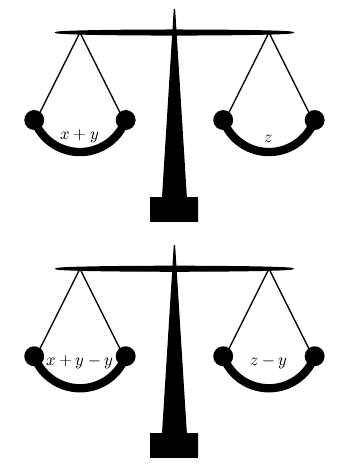
\includegraphics[height=300px]{col11306.imgs/m38346_MG10C2_002.png} % m38346;MG10C2\_002.png;;;6.0;8.5;
      \vspace{2pt}
    \vspace{\rubberspace}\par \begin{cnxcaption}
	  \small \textbf{Figure 2: }An equation is like a set of weighing scales. In order to keep the
scales balanced, you must do the same thing to both sides. So, if you add,
subtract, multiply or divide the one side, you must add, subtract, multiply or
divide the other side too.
	\end{cnxcaption}
    \vspace{.1in}
    \rule[.1in]{\figurerulewidth}{.005in} \\
    \end{center}
 \end{figure}       
      \label{m38346*uid38}
            \subsection{ Method: Rearranging Equations}
            \nopagebreak
        \label{m38346*id176160}You can add, subtract, multiply or divide both sides of an equation by any
number you want, as long as you always do it to both sides.\par 
        \label{m38346*id176164}So for our example we could subtract $y$ from both sides\par 
        \label{m38346*uid39}\nopagebreak\noindent{}
          \settowidth{\mymathboxwidth}{\begin{equation}
    \begin{array}{ccc}\hfill x+y& =& z\hfill \\ \hfill x+y-y& =& z-y\hfill \\ \hfill x& =& z-y\hfill \\ \hfill x& =& 15-10\hfill \\ \hfill & =& 5\hfill \end{array}\tag{26}
      \end{equation}
    }
    \typeout{Columnwidth = \the\columnwidth}\typeout{math as usual width = \the\mymathboxwidth}
    \ifthenelse{\lengthtest{\mymathboxwidth < \columnwidth}}{% if the math fits, do it again, for real
    \begin{equation}
    \begin{array}{ccc}\hfill x+y& =& z\hfill \\ \hfill x+y-y& =& z-y\hfill \\ \hfill x& =& z-y\hfill \\ \hfill x& =& 15-10\hfill \\ \hfill & =& 5\hfill \end{array}\tag{26}
      \end{equation}
    }{% else, if it doesn't fit
    \setlength{\mymathboxwidth}{\columnwidth}
      \addtolength{\mymathboxwidth}{-48pt}
    \par\vspace{12pt}\noindent\begin{minipage}{\columnwidth}
    \parbox[t]{\mymathboxwidth}{\large$
    x+y=zx+y-y=z-yx=z-yx=15-10=5$}\hfill
    \parbox[t]{48pt}{\raggedleft 
    (26)}
    \end{minipage}\vspace{12pt}\par
    }% end of conditional for this bit of math
    \typeout{math as usual width = \the\mymathboxwidth}
        \label{m38346*id176299}Now we can see that the change is the price subtracted from the amount paid
to the cashier. In the example, the change should be R5. In real life we
can do this in our heads; the human brain is very smart and can do arithmetic
without even knowing it.\par 
        \label{m38346*id176307}When you subtract a number from both sides of an equation, it looks like
you just moved a positive number from one side and it became a negative on the other,
which is exactly what happened. Likewise, if you move a multiplied number from
one side to the other, it looks like it changed to a divide. This is because you
really just divided both sides by that number and a number divided by itself is
just 1\par 
        \label{m38346*uid40}\nopagebreak\noindent{}
          \settowidth{\mymathboxwidth}{\begin{equation}
    \begin{array}{ccc}\hfill a\left(5+c\right)& =& 3a\hfill \\ \hfill a\left(5+c\right)÷a& =& 3a÷a\hfill \\ \hfill \frac{a}{a}\ensuremath{\times}\left(5+c\right)& =& 3\ensuremath{\times}\frac{a}{a}\hfill \\ \hfill 1\ensuremath{\times}\left(5+c\right)& =& 3\ensuremath{\times}1\hfill \\ \hfill 5+c& =& 3\hfill \\ \hfill c& =& 3-5=-2\hfill \end{array}\tag{27}
      \end{equation}
    }
    \typeout{Columnwidth = \the\columnwidth}\typeout{math as usual width = \the\mymathboxwidth}
    \ifthenelse{\lengthtest{\mymathboxwidth < \columnwidth}}{% if the math fits, do it again, for real
    \begin{equation}
    \begin{array}{ccc}\hfill a\left(5+c\right)& =& 3a\hfill \\ \hfill a\left(5+c\right)÷a& =& 3a÷a\hfill \\ \hfill \frac{a}{a}\ensuremath{\times}\left(5+c\right)& =& 3\ensuremath{\times}\frac{a}{a}\hfill \\ \hfill 1\ensuremath{\times}\left(5+c\right)& =& 3\ensuremath{\times}1\hfill \\ \hfill 5+c& =& 3\hfill \\ \hfill c& =& 3-5=-2\hfill \end{array}\tag{27}
      \end{equation}
    }{% else, if it doesn't fit
    \setlength{\mymathboxwidth}{\columnwidth}
      \addtolength{\mymathboxwidth}{-48pt}
    \par\vspace{12pt}\noindent\begin{minipage}{\columnwidth}
    \parbox[t]{\mymathboxwidth}{\large$
    a\left(5+c\right)=3aa\left(5+c\right)÷a=3a÷a\frac{a}{a}\ensuremath{\times}\left(5+c\right)=3\ensuremath{\times}\frac{a}{a}1\ensuremath{\times}\left(5+c\right)=3\ensuremath{\times}15+c=3c=3-5=-2$}\hfill
    \parbox[t]{48pt}{\raggedleft 
    (27)}
    \end{minipage}\vspace{12pt}\par
    }% end of conditional for this bit of math
    \typeout{math as usual width = \the\mymathboxwidth}
        \label{m38346*id176526}However, you must be careful when doing this, as it is easy to make mistakes.\par 
        \label{m38346*id176532}
          \textbf{The following is the WRONG thing to do}
        \par 
        \label{m38346*uid41}\nopagebreak\noindent{}
          \settowidth{\mymathboxwidth}{\begin{equation}
    \begin{array}{ccc}\hfill 5a+c& =& 3a\hfill \\ \hfill 5+c& =& 3\hfill \end{array}\tag{28}
      \end{equation}
    }
    \typeout{Columnwidth = \the\columnwidth}\typeout{math as usual width = \the\mymathboxwidth}
    \ifthenelse{\lengthtest{\mymathboxwidth < \columnwidth}}{% if the math fits, do it again, for real
    \begin{equation}
    \begin{array}{ccc}\hfill 5a+c& =& 3a\hfill \\ \hfill 5+c& =& 3\hfill \end{array}\tag{28}
      \end{equation}
    }{% else, if it doesn't fit
    \setlength{\mymathboxwidth}{\columnwidth}
      \addtolength{\mymathboxwidth}{-48pt}
    \par\vspace{12pt}\noindent\begin{minipage}{\columnwidth}
    \parbox[t]{\mymathboxwidth}{\large$
    5a+c=3a5+c=3$}\hfill
    \parbox[t]{48pt}{\raggedleft 
    (28)}
    \end{minipage}\vspace{12pt}\par
    }% end of conditional for this bit of math
    \typeout{math as usual width = \the\mymathboxwidth}
        \label{m38346*id176602}Can you see why it is wrong? It is wrong because we did not divide the $c$ term
by $a$ as well. The correct thing to do is\par 
        \label{m38346*uid42}\nopagebreak\noindent{}
          \settowidth{\mymathboxwidth}{\begin{equation}
    \begin{array}{ccc}\hfill 5a+c& =& 3a\hfill \\ \hfill 5+c÷a& =& 3\hfill \\ \hfill c÷a& =& 3-5=-2\hfill \end{array}\tag{29}
      \end{equation}
    }
    \typeout{Columnwidth = \the\columnwidth}\typeout{math as usual width = \the\mymathboxwidth}
    \ifthenelse{\lengthtest{\mymathboxwidth < \columnwidth}}{% if the math fits, do it again, for real
    \begin{equation}
    \begin{array}{ccc}\hfill 5a+c& =& 3a\hfill \\ \hfill 5+c÷a& =& 3\hfill \\ \hfill c÷a& =& 3-5=-2\hfill \end{array}\tag{29}
      \end{equation}
    }{% else, if it doesn't fit
    \setlength{\mymathboxwidth}{\columnwidth}
      \addtolength{\mymathboxwidth}{-48pt}
    \par\vspace{12pt}\noindent\begin{minipage}{\columnwidth}
    \parbox[t]{\mymathboxwidth}{\large$
    5a+c=3a5+c÷a=3c÷a=3-5=-2$}\hfill
    \parbox[t]{48pt}{\raggedleft 
    (29)}
    \end{minipage}\vspace{12pt}\par
    }% end of conditional for this bit of math
    \typeout{math as usual width = \the\mymathboxwidth}
\label{m38346*secfhsst!!!underscore!!!id1732}
            \subsubsection{  Rearranging Equations }
            \nopagebreak
        \label{m38346*id176734}\begin{enumerate}[noitemsep, label=\textbf{\arabic*}. ] 
            \label{m38346*uid43}\item If $3\left(2r-5\right)=27$, then $2r-5=.....$\hspace{1ex}        \label{m38346*uid44}\item Find the value for $x$ if $0,5\left(x-8\right)=0,2x+11$\hspace{1ex}        \label{m38346*uid45}\item Solve $9-2n=3\left(n+2\right)$\hspace{1ex}        \label{m38346*uid46}\item Change the formula $P=A+Akt$ \hspace{1ex}to $A=$\hspace{1ex}        \label{m38346*uid47}\item Solve for $x$: $\frac{1}{ax}+\frac{1}{bx}=1$\hspace{1ex}        \end{enumerate}
\par \raisebox{-5 pt}{
\includegraphics[width=0.5cm]{col11306.imgs/summary_www.png}} Find the answers with the shortcodes:
 \par \begin{tabular}[h]{cccccc}
 (1.) l3k  &  (2.) l30  &  (3.) l38  &  (4.) l39  &  (5.) l3X  & \end{tabular}
    \section{Fractions and Decimal Numbers}
            \nopagebreak
%%            \label{m38346*cid11} $ \hspace{-5pt}\begin{array}{cccccccccccc}   \end{array} $ \hspace{2 pt}\raisebox{-5 pt}{
\includegraphics[width=0.5cm]{col11306.imgs/summary_www.png}} {(section shortcode: MG10009 )} \par 
      \label{m38346*id177025}A fraction is one number divided by another number. There are several ways to
write a number divided by another one, such as $a÷b$, $a/b$ and $\frac{a}{b}$.
The first way of writing a fraction is very hard to work with, so we will use
only the other two. We call the number on the top (left) the \textsl{numerator} and
the number on the bottom (right) the \textsl{denominator}. For example, in the fraction
$1/5$ or $\frac{1}{5}$, the numerator is 1 and the denominator is 5.\par 
\label{m38346*secfhsst!!!underscore!!!id1752}
            \subsection{  Definition - Fraction }
            \nopagebreak
      \label{m38346*id177118}The word \textsl{fraction} means \textsl{part
of a whole}. \par 
      \label{m38346*id177140}The \textsl{reciprocal} of a fraction is the fraction turned upside down, in
other words the numerator becomes the denominator and the denominator becomes
the numerator. So, the reciprocal of $\frac{2}{3}$ is $\frac{3}{2}$.\par 
      \label{m38346*id177178}A fraction multiplied by its reciprocal is always equal to 1 and can be
written\par 
      \label{m38346*uid48}\nopagebreak\noindent{}
        \settowidth{\mymathboxwidth}{\begin{equation}
    \frac{a}{b}\ensuremath{\times}\frac{b}{a}=1\tag{30}
      \end{equation}
    }
    \typeout{Columnwidth = \the\columnwidth}\typeout{math as usual width = \the\mymathboxwidth}
    \ifthenelse{\lengthtest{\mymathboxwidth < \columnwidth}}{% if the math fits, do it again, for real
    \begin{equation}
    \frac{a}{b}\ensuremath{\times}\frac{b}{a}=1\tag{30}
      \end{equation}
    }{% else, if it doesn't fit
    \setlength{\mymathboxwidth}{\columnwidth}
      \addtolength{\mymathboxwidth}{-48pt}
    \par\vspace{12pt}\noindent\begin{minipage}{\columnwidth}
    \parbox[t]{\mymathboxwidth}{\large$
    \frac{a}{b}\ensuremath{\times}\frac{b}{a}=1$}\hfill
    \parbox[t]{48pt}{\raggedleft 
    (30)}
    \end{minipage}\vspace{12pt}\par
    }% end of conditional for this bit of math
    \typeout{math as usual width = \the\mymathboxwidth}
      \label{m38346*id177217}This is because dividing by a number is the same as multiplying by its
reciprocal.\par 
\label{m38346*secfhsst!!!underscore!!!id1780}
            \subsection{  Definition - Multiplicative Inverse }
            \nopagebreak
      \label{m38346*id177229}The reciprocal of a number is
also known as the multiplicative inverse. \par 
      \label{m38346*id177241}A decimal number is a number which has an integer part and a fractional part.
The integer and the fractional parts are separated by a \textsl{decimal point},
which is written as a comma in South African schools. For example the number $3\frac{14}{100}$ can be written much more neatly as $3,14$.\par 
      \label{m38346*id177283}All real numbers can be written as a decimal number. However, some numbers would
take a huge amount of paper (and ink) to write out in full! Some decimal numbers
will have a number which will repeat itself, such as $0,33333...$ where there
are an infinite number of 3's. We can write this decimal value by using a dot
above the repeating number, so $0,\dot{3}=0,33333...$. If there are two
repeating numbers such as $0,121212...$ then you can place dots\label{m38346*uid49}\footnote{or a
bar, like $0,\overline{12}$} on each of the repeated numbers
$0,\dot{1}\dot{2}=0,121212...$. These kinds of repeating decimals are called
\textsl{recurring decimals}.\par 
      \label{m38346*id177428}Table 5 lists some common fractions and their
decimal forms.\par 
    % \textbf{m38346*uid50}\par
          \begin{table}
    % \begin{table}[H]
    % \\ '' '0'
        \begin{center}
      \label{m38346*uid50}
    \noindent
    \tabletail{%
        \hline
        \multicolumn{2}{|p{\mytableboxwidth}|}{\raggedleft \small \sl continued on next page}\\
        \hline
      }
      \tablelasttail{}
      \begin{xtabular}[t]{|l|l|}\hline
        Fraction &
        Decimal Form% make-rowspan-placeholders
     \tabularnewline\cline{1-1}\cline{2-2}
      %--------------------------------------------------------------------
                $\frac{1}{20}$
               &
        0,05% make-rowspan-placeholders
     \tabularnewline\cline{1-1}\cline{2-2}
      %--------------------------------------------------------------------
                $\frac{1}{16}$
               &
        0,0625% make-rowspan-placeholders
     \tabularnewline\cline{1-1}\cline{2-2}
      %--------------------------------------------------------------------
                $\frac{1}{10}$
               &
        0,1% make-rowspan-placeholders
     \tabularnewline\cline{1-1}\cline{2-2}
      %--------------------------------------------------------------------
                $\frac{1}{8}$
               &
        0,125% make-rowspan-placeholders
     \tabularnewline\cline{1-1}\cline{2-2}
      %--------------------------------------------------------------------
                $\frac{1}{6}$
               &
                $0,16\dot{6}$
              % make-rowspan-placeholders
     \tabularnewline\cline{1-1}\cline{2-2}
      %--------------------------------------------------------------------
                $\frac{1}{5}$
               &
        0,2% make-rowspan-placeholders
     \tabularnewline\cline{1-1}\cline{2-2}
      %--------------------------------------------------------------------
                $\frac{1}{2}$
               &
        0,5% make-rowspan-placeholders
     \tabularnewline\cline{1-1}\cline{2-2}
      %--------------------------------------------------------------------
                $\frac{3}{4}$
               &
        0,75% make-rowspan-placeholders
     \tabularnewline\cline{1-1}\cline{2-2}
      %--------------------------------------------------------------------
    \end{xtabular}
      \end{center}
    \begin{center}{\small\bfseries Table 5}: Some common fractions and their equivalent decimal forms.\end{center}
    \begin{caption}{\small\bfseries Table 5}: Some common fractions and their equivalent decimal forms.\end{caption}
\end{table}
    \par
    \section{Scientific Notation}
            \nopagebreak
%%            \label{m38346*cid12} $ \hspace{-5pt}\begin{array}{cccccccccccc}   \end{array} $ \hspace{2 pt}\raisebox{-5 pt}{
\includegraphics[width=0.5cm]{col11306.imgs/summary_www.png}} {(section shortcode: MG10010 )} \par 
      \label{m38346*id177822}In science one often needs to work with very large or very small numbers. These
can be written more easily in scientific notation, which has the general form\par 
      \label{m38346*uid51}\nopagebreak\noindent{}
        \settowidth{\mymathboxwidth}{\begin{equation}
    a\ensuremath{\times}{10}^{m}\tag{31}
      \end{equation}
    }
    \typeout{Columnwidth = \the\columnwidth}\typeout{math as usual width = \the\mymathboxwidth}
    \ifthenelse{\lengthtest{\mymathboxwidth < \columnwidth}}{% if the math fits, do it again, for real
    \begin{equation}
    a\ensuremath{\times}{10}^{m}\tag{31}
      \end{equation}
    }{% else, if it doesn't fit
    \setlength{\mymathboxwidth}{\columnwidth}
      \addtolength{\mymathboxwidth}{-48pt}
    \par\vspace{12pt}\noindent\begin{minipage}{\columnwidth}
    \parbox[t]{\mymathboxwidth}{\large$
    a\ensuremath{\times}{10}^{m}$}\hfill
    \parbox[t]{48pt}{\raggedleft 
    (31)}
    \end{minipage}\vspace{12pt}\par
    }% end of conditional for this bit of math
    \typeout{math as usual width = \the\mymathboxwidth}
      \label{m38346*id177854}where $a$ is a decimal number between 0 and 10 that is rounded off to a few
decimal places. The $m$ is an integer and if it is positive it represents how
many zeros should appear to the right of $a$. If $m$ is negative, then it
represents how many times the decimal place in $a$ should be moved to the left.
For example $3,2\ensuremath{\times}{10}^{3}$ represents 32~000 and $3,2\ensuremath{\times}{10}^{-3}$ represents
$0,0032$.\par 
      \label{m38346*id177971}If a number must be converted into scientific notation, we need to work out how
many times the number must be multiplied or divided by 10 to make it into a
number between 1 and 10 (i.e. we need to work out the value of the exponent $m$)
and what this number is (the value of $a$). We do this by counting the number of
decimal places the decimal point must move.\par 
      \label{m38346*id177995}For example, write the speed of light which is $299 792 458\phantom{\rule{3pt}{0ex}}m\ensuremath{\cdot}s{}^{-1}$ in
scientific notation, to two decimal places. First, determine where the decimal
point must go for two decimal places (to find $a$) and then count how many
places there are after the decimal point to determine $m$.\par 
      \label{m38346*id178035}In this example, the decimal point must go after the first 2, but since the
number after the 9 is a 7, $a=3,00$.\par 
      \label{m38346*id178057}So the number is $3,00\ensuremath{\times}{10}^{m}$, where $m=8$, because there are 8 digits
left after the decimal point. So, the speed of light in scientific notation to
two decimal places is $3,00\ensuremath{\times}{10}^{8}\phantom{\rule{3pt}{0ex}}m\ensuremath{\cdot}s{}^{-1}$\par 
      \label{m38346*id178140}As another example, the size of the HI virus is around $1,2\ensuremath{\times}{10}^{-7}$~m.
This is equal to $1,2\ensuremath{\times}0,0000001\phantom{\rule{3pt}{0ex}}m$, which is $0,00000012\phantom{\rule{3pt}{0ex}}m$.\par 
    \section{Real Numbers}
            \nopagebreak
%%            \label{m38346*cid13} $ \hspace{-5pt}\begin{array}{cccccccccccc}   \end{array} $ \hspace{2 pt}\raisebox{-5 pt}{
\includegraphics[width=0.5cm]{col11306.imgs/summary_www.png}} {(section shortcode: MG10011 )} \par 
      \label{m38346*id178203}Now that we have learnt about the basics of mathematics, we can look at what
real numbers are in a little more detail. The following are examples of real
numbers and it is seen that each number is written in a different way.\par 
      \label{m38346*uid52}\nopagebreak\noindent{}
        \settowidth{\mymathboxwidth}{\begin{equation}
    \sqrt{3},1,2557878,\frac{56}{34},10,2,1,-5,-6,35,-\frac{1}{90}\tag{32}
      \end{equation}
    }
    \typeout{Columnwidth = \the\columnwidth}\typeout{math as usual width = \the\mymathboxwidth}
    \ifthenelse{\lengthtest{\mymathboxwidth < \columnwidth}}{% if the math fits, do it again, for real
    \begin{equation}
    \sqrt{3},1,2557878,\frac{56}{34},10,2,1,-5,-6,35,-\frac{1}{90}\tag{32}
      \end{equation}
    }{% else, if it doesn't fit
    \setlength{\mymathboxwidth}{\columnwidth}
      \addtolength{\mymathboxwidth}{-48pt}
    \par\vspace{12pt}\noindent\begin{minipage}{\columnwidth}
    \parbox[t]{\mymathboxwidth}{\large$
    \sqrt{3},1,2557878,\frac{56}{34},10,2,1,-5,-6,35,-\frac{1}{90}$}\hfill
    \parbox[t]{48pt}{\raggedleft 
    (32)}
    \end{minipage}\vspace{12pt}\par
    }% end of conditional for this bit of math
    \typeout{math as usual width = \the\mymathboxwidth}
      \label{m38346*id178306}Depending on how the real number is written, it can be further labelled as
either rational, irrational, integer or natural. A set diagram of the different
number types is shown in Figure~3.\par 
    \setcounter{subfigure}{0}
	\begin{figure}[H] % horizontal\label{m38346*uid53}
    \begin{center}
    \rule[.1in]{\figurerulewidth}{.005in} \\
        \label{m38346*uid53!!!underscore!!!media}\label{m38346*uid53!!!underscore!!!printimage}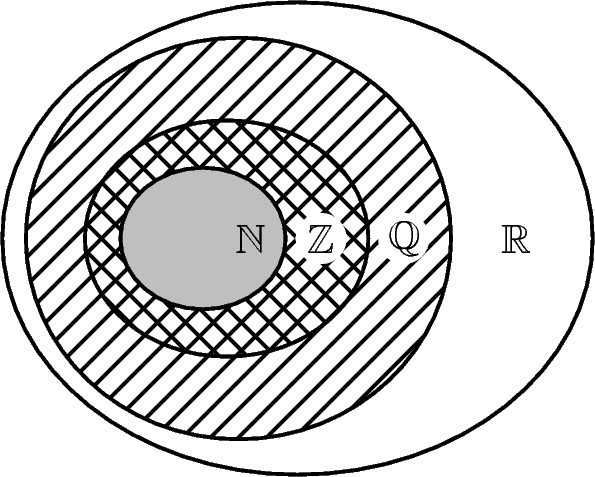
\includegraphics{col11306.imgs/m38346_MG10C2_003.png} % m38346;MG10C2\_003.png;;;6.0;8.5;
      \vspace{2pt}
    \vspace{\rubberspace}\par \begin{cnxcaption}
	  \small \textbf{Figure 3: }Set diagram of all the real numbers $\mathbb{R}$, the rational
numbers $\mathbb{Q}$, the integers $\mathbb{Z}$ and the natural numbers $\mathbb{N}$. The irrational numbers are the numbers not inside the set of rational
numbers. All of the integers are also rational numbers, but not all rational
numbers are integers.
	\end{cnxcaption}
    \vspace{.1in}
    \rule[.1in]{\figurerulewidth}{.005in} \\
    \end{center}
 \end{figure}       
\label{m38346*secfhsst!!!underscore!!!id2036}
            \subsection{  Non-Real Numbers }
            \nopagebreak
      \label{m38346*id178383}All numbers that are not real numbers have
\textsl{imaginary} components. We will not see imaginary numbers in this book
but they come from $\sqrt{-1}$. Since we won't be looking at
numbers which are not real, if you see a number you can be sure it is a real
one. \par 
      \label{m38346*uid54}
            \subsection{ Natural Numbers}
            \nopagebreak
        \label{m38346*id178423}The first type of numbers that are learnt about are the numbers that are used
for counting. These numbers are called \textsl{natural numbers} and are the
simplest numbers in mathematics:\par 
        \label{m38346*uid55}\nopagebreak\noindent{}
          \settowidth{\mymathboxwidth}{\begin{equation}
    0,1,2,3,4,...\tag{33}
      \end{equation}
    }
    \typeout{Columnwidth = \the\columnwidth}\typeout{math as usual width = \the\mymathboxwidth}
    \ifthenelse{\lengthtest{\mymathboxwidth < \columnwidth}}{% if the math fits, do it again, for real
    \begin{equation}
    0,1,2,3,4,...\tag{33}
      \end{equation}
    }{% else, if it doesn't fit
    \setlength{\mymathboxwidth}{\columnwidth}
      \addtolength{\mymathboxwidth}{-48pt}
    \par\vspace{12pt}\noindent\begin{minipage}{\columnwidth}
    \parbox[t]{\mymathboxwidth}{\large$
    0,1,2,3,4,...$}\hfill
    \parbox[t]{48pt}{\raggedleft 
    (33)}
    \end{minipage}\vspace{12pt}\par
    }% end of conditional for this bit of math
    \typeout{math as usual width = \the\mymathboxwidth}
        \label{m38346*id178472}Mathematicians use the symbol ${\mathbb{N}}_{0}$ to mean the \textsl{set of all natural
numbers}. These are also sometimes called \textsl{whole numbers}. The natural numbers are a \textsl{subset} of the real numbers since
every natural number is also a real number.\par 
      \label{m38346*uid56}
            \subsection{ Integers}
            \nopagebreak
        \label{m38346*id178521}The integers are all of the natural numbers and their negatives:\par 
        \label{m38346*uid57}\nopagebreak\noindent{}
          \settowidth{\mymathboxwidth}{\begin{equation}
    ...-4,-3,-2,-1,0,1,2,3,4...\tag{34}
      \end{equation}
    }
    \typeout{Columnwidth = \the\columnwidth}\typeout{math as usual width = \the\mymathboxwidth}
    \ifthenelse{\lengthtest{\mymathboxwidth < \columnwidth}}{% if the math fits, do it again, for real
    \begin{equation}
    ...-4,-3,-2,-1,0,1,2,3,4...\tag{34}
      \end{equation}
    }{% else, if it doesn't fit
    \setlength{\mymathboxwidth}{\columnwidth}
      \addtolength{\mymathboxwidth}{-48pt}
    \par\vspace{12pt}\noindent\begin{minipage}{\columnwidth}
    \parbox[t]{\mymathboxwidth}{\large$
    ...-4,-3,-2,-1,0,1,2,3,4...$}\hfill
    \parbox[t]{48pt}{\raggedleft 
    (34)}
    \end{minipage}\vspace{12pt}\par
    }% end of conditional for this bit of math
    \typeout{math as usual width = \the\mymathboxwidth}
        \label{m38346*id178589}Mathematicians use the symbol $\mathbb{Z}$ to mean \textsl{the set of all
integers}. The integers are a subset of the real numbers, since every integer is
a real number.\par 
      \label{m38346*uid58}
            \subsection{ Rational Numbers}
            \nopagebreak
        \label{m38346*id178622}The natural numbers and the integers are only able to describe quantities that
are whole or complete. For example, you can have 4 apples, but what happens when
you divide one apple into 4 equal pieces and share it among your friends? Then
it is not a whole apple anymore and a different type of number is needed to
describe the apples. This type of number is known as a rational number.\par 
        \label{m38346*id178628}A rational number is any number which can be written as:\par 
        \label{m38346*uid59}\nopagebreak\noindent{}
          \settowidth{\mymathboxwidth}{\begin{equation}
    \frac{a}{b}\tag{35}
      \end{equation}
    }
    \typeout{Columnwidth = \the\columnwidth}\typeout{math as usual width = \the\mymathboxwidth}
    \ifthenelse{\lengthtest{\mymathboxwidth < \columnwidth}}{% if the math fits, do it again, for real
    \begin{equation}
    \frac{a}{b}\tag{35}
      \end{equation}
    }{% else, if it doesn't fit
    \setlength{\mymathboxwidth}{\columnwidth}
      \addtolength{\mymathboxwidth}{-48pt}
    \par\vspace{12pt}\noindent\begin{minipage}{\columnwidth}
    \parbox[t]{\mymathboxwidth}{\large$
    \frac{a}{b}$}\hfill
    \parbox[t]{48pt}{\raggedleft 
    (35)}
    \end{minipage}\vspace{12pt}\par
    }% end of conditional for this bit of math
    \typeout{math as usual width = \the\mymathboxwidth}
        \label{m38346*id178652}where $a$ and $b$ are integers and $b\ne 0$.\par 
        \label{m38346*id178690}The following are examples of rational numbers:\par 
        \label{m38346*uid60}\nopagebreak\noindent{}
          \settowidth{\mymathboxwidth}{\begin{equation}
    \frac{20}{9},\frac{-1}{2},\frac{20}{10},\frac{3}{15}\tag{36}
      \end{equation}
    }
    \typeout{Columnwidth = \the\columnwidth}\typeout{math as usual width = \the\mymathboxwidth}
    \ifthenelse{\lengthtest{\mymathboxwidth < \columnwidth}}{% if the math fits, do it again, for real
    \begin{equation}
    \frac{20}{9},\frac{-1}{2},\frac{20}{10},\frac{3}{15}\tag{36}
      \end{equation}
    }{% else, if it doesn't fit
    \setlength{\mymathboxwidth}{\columnwidth}
      \addtolength{\mymathboxwidth}{-48pt}
    \par\vspace{12pt}\noindent\begin{minipage}{\columnwidth}
    \parbox[t]{\mymathboxwidth}{\large$
    \frac{20}{9},\frac{-1}{2},\frac{20}{10},\frac{3}{15}$}\hfill
    \parbox[t]{48pt}{\raggedleft 
    (36)}
    \end{minipage}\vspace{12pt}\par
    }% end of conditional for this bit of math
    \typeout{math as usual width = \the\mymathboxwidth}
\label{m38346*secfhsst!!!underscore!!!id2154}
            \subsubsection{  Notation Tip }
            \nopagebreak
        \label{m38346*id178758}Rational numbers are any number that can be expressed
in the form $\frac{a}{b};a,b\in \mathbb{Z};b\ne 0$ which means ``the set of
numbers $\frac{a}{b}$ when $a$ and $b$ are integers''. \par 
        \label{m38346*id178840}Mathematicians use the symbol $\mathbb{Q}$ to mean \textsl{the set of all
rational numbers}. The set of rational numbers contains all numbers which can be
written as terminating or repeating decimals.\par 
\label{m38346*secfhsst!!!underscore!!!id2162}
            \subsubsection{  Rational Numbers }
            \nopagebreak
        \label{m38346*id178867}All integers are rational numbers with a denominator of
1. \par 
        \label{m38346*id178879}You can add and multiply rational numbers and still get a rational number at the
end, which is very useful. If we have 4 integers $a,b,c$ and $d$, then the
rules for adding and multiplying rational numbers are
\par 
        \label{m38346*uid61}\nopagebreak\noindent{}
          \settowidth{\mymathboxwidth}{\begin{equation}
    \begin{array}{ccc}\hfill \frac{a}{b}+\frac{c}{d}& =& \frac{ad+bc}{bd}\hfill \\ \hfill \frac{a}{b}\ensuremath{\times}\frac{c}{d}& =& \frac{ac}{bd}\hfill \end{array}\tag{37}
      \end{equation}
    }
    \typeout{Columnwidth = \the\columnwidth}\typeout{math as usual width = \the\mymathboxwidth}
    \ifthenelse{\lengthtest{\mymathboxwidth < \columnwidth}}{% if the math fits, do it again, for real
    \begin{equation}
    \begin{array}{ccc}\hfill \frac{a}{b}+\frac{c}{d}& =& \frac{ad+bc}{bd}\hfill \\ \hfill \frac{a}{b}\ensuremath{\times}\frac{c}{d}& =& \frac{ac}{bd}\hfill \end{array}\tag{37}
      \end{equation}
    }{% else, if it doesn't fit
    \setlength{\mymathboxwidth}{\columnwidth}
      \addtolength{\mymathboxwidth}{-48pt}
    \par\vspace{12pt}\noindent\begin{minipage}{\columnwidth}
    \parbox[t]{\mymathboxwidth}{\large$
    \frac{a}{b}+\frac{c}{d}=\frac{ad+bc}{bd}\frac{a}{b}\ensuremath{\times}\frac{c}{d}=\frac{ac}{bd}$}\hfill
    \parbox[t]{48pt}{\raggedleft 
    (37)}
    \end{minipage}\vspace{12pt}\par
    }% end of conditional for this bit of math
    \typeout{math as usual width = \the\mymathboxwidth}
\label{m38346*secfhsst!!!underscore!!!id2239}
            \subsubsection{  Notation Tip }
            \nopagebreak
        \label{m38346*id179027}The statement "4 integers $a,b,c$ and $d$" can be
written formally as $\{a,b,c,d\}\in \mathbb{Z}$ because the $\in $ symbol means
\textsl{in} and we say that $a,b,c$ and $d$ are \textsl{in} the set of
integers. \par 
        \label{m38346*id179148}Two rational numbers ($\frac{a}{b}$ and $\frac{c}{d}$) represent the same number if $ad=bc$. It is always best to simplify any rational number, so that the
denominator is as small as possible. This can be achieved by dividing both the numerator and the denominator by the same integer. For example, the rational number $1000/10000$ can be divided by 1000 on the top and the bottom, which gives $1/10$. $\frac{2}{3}$ of a pizza is the same as $\frac{8}{12}$ (Figure~4).\par 
    \setcounter{subfigure}{0}
	\begin{figure}[H] % horizontal\label{m38346*uid62}
    \begin{center}
    \rule[.1in]{\figurerulewidth}{.005in} \\
        \label{m38346*uid62!!!underscore!!!media}\label{m38346*uid62!!!underscore!!!printimage}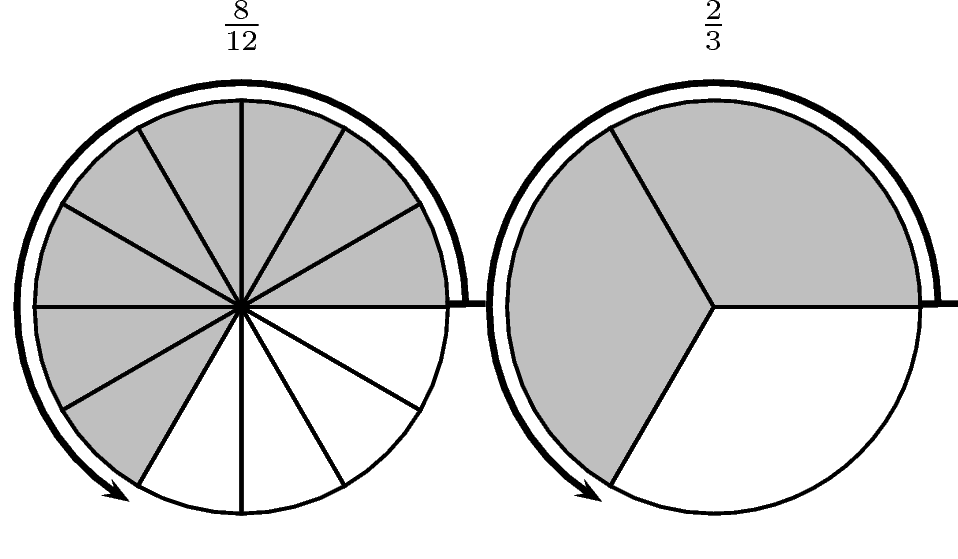
\includegraphics{col11306.imgs/m38346_MG10C2_004.png} % m38346;MG10C2\_004.png;;;6.0;8.5;
      \vspace{2pt}
    \vspace{\rubberspace}\par \begin{cnxcaption}
	  \small \textbf{Figure 4: }$\frac{8}{12}$ of the pizza is the same as $\frac{2}{3}$ of the pizza.
	\end{cnxcaption}
    \vspace{.1in}
    \rule[.1in]{\figurerulewidth}{.005in} \\
    \end{center}
 \end{figure}       
        \label{m38346*id179295}You can also add rational numbers together by finding the \textsl{lowest common denominator} and then adding the numerators. Finding a lowest common
denominator means finding the lowest number that both denominators are a
\textsl{factor}\label{m38346*uid63}\footnote{Some people say \textsl{divisor} instead of factor.}
of. A factor of a number is an integer which evenly divides that number without
leaving a remainder. The following numbers all have a factor of 3\par 
        \label{m38346*id179327}\nopagebreak\noindent{}
          \settowidth{\mymathboxwidth}{\begin{equation}
    3,6,9,12,15,18,21,24,...\tag{38}
      \end{equation}
    }
    \typeout{Columnwidth = \the\columnwidth}\typeout{math as usual width = \the\mymathboxwidth}
    \ifthenelse{\lengthtest{\mymathboxwidth < \columnwidth}}{% if the math fits, do it again, for real
    \begin{equation}
    3,6,9,12,15,18,21,24,...\tag{38}
      \end{equation}
    }{% else, if it doesn't fit
    \setlength{\mymathboxwidth}{\columnwidth}
      \addtolength{\mymathboxwidth}{-48pt}
    \par\vspace{12pt}\noindent\begin{minipage}{\columnwidth}
    \parbox[t]{\mymathboxwidth}{\large$
    3,6,9,12,15,18,21,24,...$}\hfill
    \parbox[t]{48pt}{\raggedleft 
    (38)}
    \end{minipage}\vspace{12pt}\par
    }% end of conditional for this bit of math
    \typeout{math as usual width = \the\mymathboxwidth}
        \label{m38346*id179373}and the following all have factors of 4\par 
        \label{m38346*id179379}\nopagebreak\noindent{}
          \settowidth{\mymathboxwidth}{\begin{equation}
    4,8,12,16,20,24,28,...\tag{39}
      \end{equation}
    }
    \typeout{Columnwidth = \the\columnwidth}\typeout{math as usual width = \the\mymathboxwidth}
    \ifthenelse{\lengthtest{\mymathboxwidth < \columnwidth}}{% if the math fits, do it again, for real
    \begin{equation}
    4,8,12,16,20,24,28,...\tag{39}
      \end{equation}
    }{% else, if it doesn't fit
    \setlength{\mymathboxwidth}{\columnwidth}
      \addtolength{\mymathboxwidth}{-48pt}
    \par\vspace{12pt}\noindent\begin{minipage}{\columnwidth}
    \parbox[t]{\mymathboxwidth}{\large$
    4,8,12,16,20,24,28,...$}\hfill
    \parbox[t]{48pt}{\raggedleft 
    (39)}
    \end{minipage}\vspace{12pt}\par
    }% end of conditional for this bit of math
    \typeout{math as usual width = \the\mymathboxwidth}
        \label{m38346*id179421}The common denominators between 3 and 4 are all the numbers that appear in both of these lists, like 12 and 24. The lowest common denominator of 3 and 4 is the smallest number that has both 3 and 4 as factors, which is 12.\par 
        \label{m38346*id179428}For example, if we wish to add $\frac{3}{4}+\frac{2}{3}$, we first need to write both fractions so that their denominators are the same by finding the lowest common denominator, which we know is 12. We can do this by multiplying $\frac{3}{4}$ by $\frac{3}{3}$ and $\frac{2}{3}$ by $\frac{4}{4}$. $\frac{3}{3}$ and $\frac{4}{4}$ are really just complicated ways of writing 1. Multiplying a number by 1 doesn't change the number.\par 
        \label{m38346*uid64}\nopagebreak\noindent{}
          \settowidth{\mymathboxwidth}{\begin{equation}
    \begin{array}{ccc}\hfill \frac{3}{4}+\frac{2}{3}& =& \frac{3}{4}\ensuremath{\times}\frac{3}{3}+\frac{2}{3}\ensuremath{\times}\frac{4}{4}\hfill \\ \hfill & =& \frac{3\ensuremath{\times}3}{4\ensuremath{\times}3}+\frac{2\ensuremath{\times}4}{3\ensuremath{\times}4}\hfill \\ \hfill & =& \frac{9}{12}+\frac{8}{12}\hfill \\ \hfill & =& \frac{9+8}{12}\hfill \\ \hfill & =& \frac{17}{12}\hfill \end{array}\tag{40}
      \end{equation}
    }
    \typeout{Columnwidth = \the\columnwidth}\typeout{math as usual width = \the\mymathboxwidth}
    \ifthenelse{\lengthtest{\mymathboxwidth < \columnwidth}}{% if the math fits, do it again, for real
    \begin{equation}
    \begin{array}{ccc}\hfill \frac{3}{4}+\frac{2}{3}& =& \frac{3}{4}\ensuremath{\times}\frac{3}{3}+\frac{2}{3}\ensuremath{\times}\frac{4}{4}\hfill \\ \hfill & =& \frac{3\ensuremath{\times}3}{4\ensuremath{\times}3}+\frac{2\ensuremath{\times}4}{3\ensuremath{\times}4}\hfill \\ \hfill & =& \frac{9}{12}+\frac{8}{12}\hfill \\ \hfill & =& \frac{9+8}{12}\hfill \\ \hfill & =& \frac{17}{12}\hfill \end{array}\tag{40}
      \end{equation}
    }{% else, if it doesn't fit
    \setlength{\mymathboxwidth}{\columnwidth}
      \addtolength{\mymathboxwidth}{-48pt}
    \par\vspace{12pt}\noindent\begin{minipage}{\columnwidth}
    \parbox[t]{\mymathboxwidth}{\large$
    \frac{3}{4}+\frac{2}{3}=\frac{3}{4}\ensuremath{\times}\frac{3}{3}+\frac{2}{3}\ensuremath{\times}\frac{4}{4}=\frac{3\ensuremath{\times}3}{4\ensuremath{\times}3}+\frac{2\ensuremath{\times}4}{3\ensuremath{\times}4}=\frac{9}{12}+\frac{8}{12}=\frac{9+8}{12}=\frac{17}{12}$}\hfill
    \parbox[t]{48pt}{\raggedleft 
    (40)}
    \end{minipage}\vspace{12pt}\par
    }% end of conditional for this bit of math
    \typeout{math as usual width = \the\mymathboxwidth}
        \label{m38346*id179732}Dividing by a rational number is the same as multiplying by its reciprocal, as long as neither the numerator nor the denominator is zero:\par 
        \label{m38346*uid65}\nopagebreak\noindent{}
          \settowidth{\mymathboxwidth}{\begin{equation}
    \frac{a}{b}÷\frac{c}{d}=\frac{a}{b}.\frac{d}{c}=\frac{ad}{bc}\tag{41}
      \end{equation}
    }
    \typeout{Columnwidth = \the\columnwidth}\typeout{math as usual width = \the\mymathboxwidth}
    \ifthenelse{\lengthtest{\mymathboxwidth < \columnwidth}}{% if the math fits, do it again, for real
    \begin{equation}
    \frac{a}{b}÷\frac{c}{d}=\frac{a}{b}.\frac{d}{c}=\frac{ad}{bc}\tag{41}
      \end{equation}
    }{% else, if it doesn't fit
    \setlength{\mymathboxwidth}{\columnwidth}
      \addtolength{\mymathboxwidth}{-48pt}
    \par\vspace{12pt}\noindent\begin{minipage}{\columnwidth}
    \parbox[t]{\mymathboxwidth}{\large$
    \frac{a}{b}÷\frac{c}{d}=\frac{a}{b}.\frac{d}{c}=\frac{ad}{bc}$}\hfill
    \parbox[t]{48pt}{\raggedleft 
    (41)}
    \end{minipage}\vspace{12pt}\par
    }% end of conditional for this bit of math
    \typeout{math as usual width = \the\mymathboxwidth}
        \label{m38346*id179798}A rational number may be a \textsl{proper} or \textsl{improper} fraction.\par 
        \label{m38346*id179812}Proper fractions have a numerator that is smaller than the denominator. For example,\par 
        \label{m38346*id179816}\nopagebreak\noindent{}
          \settowidth{\mymathboxwidth}{\begin{equation}
    \frac{-1}{2},\frac{3}{15},\frac{-5}{-20}\tag{42}
      \end{equation}
    }
    \typeout{Columnwidth = \the\columnwidth}\typeout{math as usual width = \the\mymathboxwidth}
    \ifthenelse{\lengthtest{\mymathboxwidth < \columnwidth}}{% if the math fits, do it again, for real
    \begin{equation}
    \frac{-1}{2},\frac{3}{15},\frac{-5}{-20}\tag{42}
      \end{equation}
    }{% else, if it doesn't fit
    \setlength{\mymathboxwidth}{\columnwidth}
      \addtolength{\mymathboxwidth}{-48pt}
    \par\vspace{12pt}\noindent\begin{minipage}{\columnwidth}
    \parbox[t]{\mymathboxwidth}{\large$
    \frac{-1}{2},\frac{3}{15},\frac{-5}{-20}$}\hfill
    \parbox[t]{48pt}{\raggedleft 
    (42)}
    \end{minipage}\vspace{12pt}\par
    }% end of conditional for this bit of math
    \typeout{math as usual width = \the\mymathboxwidth}
        \label{m38346*id179860}are proper fractions.\par 
        \label{m38346*id179865}Improper fractions have a numerator that is larger than the denominator. For example,\par 
        \label{m38346*id179869}\nopagebreak\noindent{}
          \settowidth{\mymathboxwidth}{\begin{equation}
    \frac{-10}{2},\frac{15}{13},\frac{-53}{-20}\tag{43}
      \end{equation}
    }
    \typeout{Columnwidth = \the\columnwidth}\typeout{math as usual width = \the\mymathboxwidth}
    \ifthenelse{\lengthtest{\mymathboxwidth < \columnwidth}}{% if the math fits, do it again, for real
    \begin{equation}
    \frac{-10}{2},\frac{15}{13},\frac{-53}{-20}\tag{43}
      \end{equation}
    }{% else, if it doesn't fit
    \setlength{\mymathboxwidth}{\columnwidth}
      \addtolength{\mymathboxwidth}{-48pt}
    \par\vspace{12pt}\noindent\begin{minipage}{\columnwidth}
    \parbox[t]{\mymathboxwidth}{\large$
    \frac{-10}{2},\frac{15}{13},\frac{-53}{-20}$}\hfill
    \parbox[t]{48pt}{\raggedleft 
    (43)}
    \end{minipage}\vspace{12pt}\par
    }% end of conditional for this bit of math
    \typeout{math as usual width = \the\mymathboxwidth}
        \label{m38346*id179913}are improper fractions. Improper fractions can always be written as the sum of an integer and a proper fraction.\par 
        \label{m38346*uid66}
            \subsubsection{ Converting Rationals into Decimal Numbers}
            \nopagebreak
          \label{m38346*id179928}Converting rationals into decimal numbers is very easy.\par 
          \label{m38346*id179931}If you use a calculator, you can simply divide the numerator by the denominator.\par 
          \label{m38346*id179935}If you do not have a calculator, then you have to use long division.\par 
          \label{m38346*id179939}Since long division was first taught in primary school, it will not be discussed here. If you have trouble with long division, then please ask your friends or your teacher to explain it to you.\par 
      \label{m38346*uid67}
            \subsection{ Irrational Numbers}
            \nopagebreak
        \label{m38346*id179954}An \textsl{irrational number} is any real number that is not a rational number. When expressed as decimals, these numbers can never be fully written out as they have an infinite number of decimal places which never fall into a repeating pattern. For example, $\sqrt{2}=1,41421356...$, $\pi =3,14159265...$. $\pi $ is a Greek letter and is pronounced ``pie''.\par 
\label{m38346*secfhsst!!!underscore!!!id2554}
            \subsubsection{  Real Numbers }
            \nopagebreak
        \label{m38346*id180025}\begin{enumerate}[noitemsep, label=\textbf{\arabic*}. ] 
            \label{m38346*uid68}\item Identify the number type (rational, irrational, real, integer) of each of the following numbers:
\label{m38346*id180040}\begin{enumerate}[noitemsep, label=\textbf{\alph*}. ] 
            \label{m38346*uid69}\item $\frac{c}{d}$ if $c$ is an integer and if $d$ is irrational.
\label{m38346*uid70}\item $\frac{3}{2}$\label{m38346*uid71}\item -25
\label{m38346*uid72}\item 1,525
\label{m38346*uid73}\item $\sqrt{10}$\end{enumerate}
                \label{m38346*uid74}\item Is the following pair of numbers real and rational or real and irrational?
Explain.
$\sqrt{4}$;$\frac{1}{8}$\hspace{1ex}        \end{enumerate}
\par \raisebox{-5 pt}{
\includegraphics[width=0.5cm]{col11306.imgs/summary_www.png}} Find the answers with the shortcodes:
 \par \begin{tabular}[h]{cccccc}
 (1.) l3b  &  (2.) l3j  & \end{tabular}
    \section{Mathematical Symbols}
            \nopagebreak
%%            \label{m38346*cid14} $ \hspace{-5pt}\begin{array}{cccccccccccc}   \end{array} $ \hspace{2 pt}\raisebox{-5 pt}{
\includegraphics[width=0.5cm]{col11306.imgs/summary_www.png}} {(section shortcode: MG10012 )} \par 
      \label{m38346*id180211}The following is a table of the meanings of some mathematical signs and symbols that you should have come across in earlier grades.\par 
    % \textbf{m38346*uid75}\par
          \begin{table}
    % \begin{table}[H]
    % \\ '' '0'
        \begin{center}
      \label{m38346*uid75}
    \noindent
    \tabletail{%
        \hline
        \multicolumn{2}{|p{\mytableboxwidth}|}{\raggedleft \small \sl continued on next page}\\
        \hline
      }
      \tablelasttail{}
      \begin{xtabular}[t]{|l|l|}\hline
        Sign or Symbol &
        Meaning% make-rowspan-placeholders
     \tabularnewline\cline{1-1}\cline{2-2}
      %--------------------------------------------------------------------
                $\greatthan{}$
               &
        greater than% make-rowspan-placeholders
     \tabularnewline\cline{1-1}\cline{2-2}
      %--------------------------------------------------------------------
                $\lessthan{}$
               &
        less than% make-rowspan-placeholders
     \tabularnewline\cline{1-1}\cline{2-2}
      %--------------------------------------------------------------------
                $\ge $
               &
        greater than or equal to% make-rowspan-placeholders
     \tabularnewline\cline{1-1}\cline{2-2}
      %--------------------------------------------------------------------
                $\le $
               &
        less than or equal to% make-rowspan-placeholders
     \tabularnewline\cline{1-1}\cline{2-2}
      %--------------------------------------------------------------------
    \end{xtabular}
      \end{center}
    \begin{center}{\small\bfseries Table 6}\end{center}
    \begin{caption}{\small\bfseries Table 6}\end{caption}
\end{table}
    \par
      \label{m38346*id180360}So if we write $x\greatthan{}5$, we say that $x$ is greater than 5 and if we write $x\ge y$, we mean that $x$ can be greater than or equal to $y$. Similarly, $\lessthan{}$ means `is less than' and $\le $ means `is less than or equal to'. Instead of saying that $x$ is between 6 and 10, we often write $6\lessthan{}x\lessthan{}10$. This directly means `six is less than $x$\hspace{1ex} which in turn is less than ten'.\par 
\label{m38346*secfhsst!!!underscore!!!id2615}
            \subsection{  Mathematical Symbols }
            \nopagebreak
      \label{m38346*id180483}\begin{enumerate}[noitemsep, label=\textbf{\arabic*}. ] 
            \label{m38346*uid76}\item Write the following in symbols:
\label{m38346*id180497}\begin{enumerate}[noitemsep, label=\textbf{\alph*}. ] 
            \label{m38346*uid77}\item $x$ is greater than 1
\label{m38346*uid78}\item $y$ is less than or equal to $z$\label{m38346*uid79}\item $a$ is greater than or equal to 21
\label{m38346*uid80}\item $p$ is greater than or equal to 21 and $p$ is less than or equal to 25
\end{enumerate}
        \hspace{1ex}        \end{enumerate}
\par \raisebox{-5 pt}{
\includegraphics[width=0.5cm]{col11306.imgs/summary_www.png}} Find the answers with the shortcodes:
 \par \begin{tabular}[h]{cccccc}
 (1.) l3I  & \end{tabular}
    \section{Infinity}
            \nopagebreak
%%            \label{m38346*cid15} $ \hspace{-5pt}\begin{array}{cccccccccccc}   \end{array} $ \hspace{2 pt}\raisebox{-5 pt}{
\includegraphics[width=0.5cm]{col11306.imgs/summary_www.png}} {(section shortcode: MG10013 )} \par 
      \label{m38346*id180617}Infinity (symbol $\infty $) is usually thought of as something like ``the largest possible number" or ``the furthest possible distance". In mathematics, infinity is often treated as if it were a number, but it is clearly a very different type of ``number" than integers or reals.\par 
      \label{m38346*id180635}When talking about recurring decimals and irrational numbers, the term \textsl{infinite} was used to describe \textsl{never-ending} digits.\par 
    \section{End of Chapter Exercises}
            \nopagebreak
%%            \label{m38346*cid16} $ \hspace{-5pt}\begin{array}{cccccccccccc}   \end{array} $ \hspace{2 pt}\raisebox{-5 pt}{
\includegraphics[width=0.5cm]{col11306.imgs/summary_www.png}} {(section shortcode: MG10014 )} \par 
      \label{m38346*id180660}\begin{enumerate}[noitemsep, label=\textbf{\arabic*}. ] 
            \label{m38346*uid81}\item Calculate
\label{m38346*id180675}\begin{enumerate}[noitemsep, label=\textbf{\alph*}. ] 
            \label{m38346*uid82}\item $18-6\ensuremath{\times}2$\label{m38346*uid83}\item $10+3\left(2+6\right)$\label{m38346*uid84}\item $50-10\left(4-2\right)+6$\label{m38346*uid85}\item $2\ensuremath{\times}9-3\left(6-1\right)+1$\label{m38346*uid86}\item $8+24÷4\ensuremath{\times}2$\label{m38346*uid87}\item $30-3\ensuremath{\times}4+2$\label{m38346*uid88}\item $36÷4\left(5-2\right)+6$\label{m38346*uid89}\item $20-4\ensuremath{\times}2+3$\label{m38346*uid90}\item $4+6\left(8+2\right)-3$\label{m38346*uid91}\item $100-10\left(2+3\right)+4$\end{enumerate}
        \hspace{1ex}        \label{m38346*uid92}\item If $p=q+4r$, then $r=.....$\hspace{1ex}        \label{m38346*uid93}\item Solve $\frac{x-2}{3}=x-3$\hspace{1ex}        \end{enumerate}
  \label{m38346**end}
\par \raisebox{-5 pt}{
\includegraphics[width=0.5cm]{col11306.imgs/summary_www.png}} Find the answers with the shortcodes:
 \par \begin{tabular}[h]{cccccc}
 (1.) l3D  &  (2.) l3W  &  (3.) l3Z  & \end{tabular}
